\documentclass[12pt,reqno]{amsart}
\usepackage{amssymb,mathrsfs,amsmath,amsfonts,amsthm,graphicx,pdfpages,MnSymbol,relsize,quiver}
\usepackage{xcolor}
\usepackage{tikz, tikz-cd}
\usepackage[section]{algorithm}
\usepackage{algorithmic}
\usepackage{wasysym}

%colors
\newcommand{\red}{{\color{red} \bullet}}
\newcommand{\green}{{\color{green} \bullet}}
\newcommand{\blue}{{\color{blue} \bullet}}
\newcommand{\define}[1]{{\bf \boldmath{#1}}}

\newcommand{\namedset}[1]{\mathbb{#1}}
\newcommand{\N}{\namedset N}

\newcommand{\X}{\mathcal{X}}
\newcommand{\Y}{\mathcal{Y}}

\newcommand{\namedcat}[1]{\mathsf{#1}}
\newcommand{\C}{\mathcal C}
\newcommand{\Cat}{\namedcat{Cat}}
\newcommand{\CMC}{\namedcat{CMC}}
\newcommand{\CMon}{\namedcat{CMon}}
\newcommand{\Mon}{\namedcat{Mon}}
\newcommand{\Set}{\namedcat{Set}}
\newcommand{\Petri}{\namedcat{Petri}}
\newcommand{\cPetri}{\namedcat{cPetri}}
\newcommand{\PSet}{\Set_{\perp}}
\newcommand{\SetPart}{\Set_{\mathrm{part}}}
\newcommand{\UNFOLD}{\mathtt{UNFOLD}}
\newcommand{\FCMon}{\mathsf{\Kl(\N)
}}
\newcommand{\Ob}{\:\mathrm{Ob}}
\newcommand{\Mor}{\:\mathrm{Mor}}
\newcommand{\Net}[1]{#1-\mathsf{Net}}
\newcommand{\Span}{\mathsf{Span}}
\newcommand{\SSpan}{\mathbb S \mathsf{pan}}
\newcommand{\CAT}{\mathsf{CAT}}
\newcommand{\im}{\mathrm{Im}\,}

\newcommand{\alphahat}{\widehat \alpha}
\newcommand{\Disp}{\mathsf{Disp}}


% \newcommand{\net}[1,2]{\begin{tikzcd}#1 \ar[r,shift left=.5ex] \ar[r,shift right=.5ex] & \N[#2] \end{tikzcd}}


\makeatletter
\newcommand*{\relrelbarsep}{.386ex}
\newcommand*{\relrelbar}{%
  \mathrel{%
    \mathpalette\@relrelbar\relrelbarsep
  }%
}
\newcommand*{\@relrelbar}[2]{%
  \raise#2\hbox to 0pt{$\m@th#1\relbar$\hss}%
  \lower#2\hbox{$\m@th#1\relbar$}%
}
\providecommand*{\rightrightarrowsfill@}{%
  \arrowfill@\relrelbar\relrelbar\rightrightarrows
}
\providecommand*{\leftleftarrowsfill@}{%
  \arrowfill@\leftleftarrows\relrelbar\relrelbar
}
\providecommand*{\xrightrightarrows}[2][]{%
  \ext@arrow 0359\rightrightarrowsfill@{#1}{#2}%
}
\providecommand*{\xleftleftarrows}[2][]{%
  \ext@arrow 3095\leftleftarrowsfill@{#1}{#2}%
}
\makeatother








%%%%%%%%%%%%%%%%%%%%%%%%%%%%%%%%%%%%%%%%%
\usepackage{subfiles}
\usepackage{stackengine}
\usepackage{mathtools}
\usepackage[utf8]{inputenc}
\usepackage{color}
\usepackage[a4paper,top=3cm,bottom=3cm,inner=3cm,outer=3cm]{geometry}

\usepackage{comment}

\usepackage{graphicx}
\usepackage{adjustbox}
\usepackage[all,2cell]{xy}\UseAllTwocells\SilentMatrices
\definecolor{darkgreen}{rgb}{0,0.45,0}
\usepackage[colorlinks,citecolor=darkgreen,urlcolor=gray,final,hyperindex,linktoc=page,pagebackref]{hyperref}
\renewcommand*{\backref}[1]{(Referred to on page #1.)}
\usepackage[capitalize]{cleveref}
\crefname{equation}{}{}
\crefname{item}{}{}
\usepackage{enumerate}



\newtheorem*{thm*}{Theorem}
\theoremstyle{remark}
\newtheorem*{rmk*}{Remark}
\newtheorem*{lem*}{Lemma}
\theoremstyle{plain}
\newtheorem*{defn*}{Definition}
\newtheorem*{cor*}{Corollary}
\theoremstyle{definition}
\newtheorem*{examples*}{Examples}
\newtheorem{prop*}{Proposition}

\theoremstyle{plain}
\newtheorem{thm}{Theorem}[section]
\theoremstyle{plain}
\newtheorem{prop}[thm]{Proposition}
\theoremstyle{remark}
\newtheorem{rmk}[thm]{Remark}
\theoremstyle{plain}
\newtheorem{lem}[thm]{Lemma}
\theoremstyle{plain}
\newtheorem{cor}[thm]{Corollary}
\theoremstyle{definition}
\newtheorem{defn}[thm]{Definition}
\theoremstyle{definition}
\newtheorem{examples}[thm]{Example}










\newcommand{\maps}{\colon}






%commenting

\newcommand{\joe}[1]{\textcolor{blue}{#1}}

\newcommand{\jade}[1]{\textcolor{purple}{#1}}
% \definecolor{purple(x11)}{rgb}{0.8, 0, 0.8}
% \def\purple{\color{purple(x11)}}
% \def\jade{\purple}




% TikZ stuff %%%%%%%%%%%%%%%%%%%%%%%%%%%%%%%%

\usetikzlibrary{arrows,positioning,fit,matrix,shapes.geometric,external}


\newcommand*\pgfdeclareanchoralias[3]{%
  \expandafter\def\csname pgf@anchor@#1@#3\expandafter\endcsname
     \expandafter{\csname pgf@anchor@#1@#2\endcsname}}

\tikzset{
    circnode/.style={
      circle, draw=red, very thin, outer sep=0.025em, minimum size=2em,
      fill=red, text centered},
    integral/.style={
      circle, draw=black, very thick, outer sep=0.025em,
      minimum size=2em, fill=blue!5, text centered},
    multiply/.style={
      circle, draw=black, very thick, outer sep=0.025em,
      minimum size=2em, fill=blue!5, text centered},
    zero/.style={
      circle, draw=black, very thick, minimum size=0.15cm, fill=black,
      inner sep=0, outer sep=0},
    bang/.style={
      circle, draw=black, very thick, minimum size=0.15cm, fill=green!10,
      inner sep=0, outer sep=0},
    delta/.style={
      regular polygon, regular polygon sides=3, minimum size=0.4cm, inner
      sep=0, outer sep=0.025em, draw=black, very thick, fill=green!10},
    codelta/.style={
      regular polygon, regular polygon sides=3, shape border rotate=180, minimum size=0.4cm,
      inner sep=0, outer sep=0.025em, draw=black, very thick, fill=green!10},
    plus/.style={
      regular polygon, regular polygon sides=3, shape border rotate=180, minimum size=0.4cm,
      inner sep = 0, outer sep=0.025em, draw=black, very thick, fill=black},
    coplus/.style={
      regular polygon, regular polygon sides=3, minimum size=0.4cm,
      inner sep = 0, outer sep=0.025em, draw=black, very thick, fill=black},
    sqnode/.style={
      regular polygon, regular polygon sides=4, minimum size=2.6em,
      draw=black, very thick, inner sep=0.2em, outer sep=0.025em,
      fill=yellow!10, text centered},
    bigcirc/.style={
      circle, draw=black, very thick, text width=1.6em, outer sep=0.025em,
      minimum height=1.6em, fill=blue!5, text centered}
}

\tikzstyle{tri}=[regular polygon,regular polygon sides=3,shape border rotate=1
80,fill=none,draw=black]

\pgfdeclareanchoralias{regular polygon}{corner 2}{left copy}
\pgfdeclareanchoralias{regular polygon}{corner 3}{right copy}
\pgfdeclareanchoralias{regular polygon}{corner 3}{addend}
\pgfdeclareanchoralias{regular polygon}{corner 2}{summand}


%TikZ


%John's Petri nets
\usepackage{tikz}
\usepackage{tikz-cd}
\usetikzlibrary{backgrounds,circuits,circuits.ee.IEC,shapes,fit,matrix}
%\tikzstyle{species}=[circle, fill=none, draw=black,scale=2]
%\tikzstyle{transition}=[rectangle, fill=none, draw=black, scale=1.5]

\def\rd{\rotatebox[origin=c]{90}{$\dashv$}} %rotate dash right
\def\ld{\rotatebox[origin=c]{-90}{$\dashv$}} %rotate dash left

\tikzstyle{simple}=[-,line width=2.000]
\tikzstyle{arrow}=[-,postaction={decorate},decoration={markings,mark=at position .5 with {\arrow{>}}},line width=1.100]
\pgfdeclarelayer{edgelayer}
\pgfdeclarelayer{nodelayer}
\pgfsetlayers{edgelayer,nodelayer,main}

\tikzstyle{none}=[inner sep=0pt]

% Petri nets
\definecolor{lblue}{rgb}{0,250,255}
\tikzstyle{species}=[circle,fill=yellow,draw=black,scale=1.15]
\tikzstyle{transition}=[rectangle,fill=lblue,draw=black,scale=1.15]
\tikzstyle{inarrow}=[->, >=stealth, shorten >=.03cm,line width=1.5]
\tikzstyle{empty}=[circle,fill=none, draw=none]
\tikzstyle{inputdot}=[circle,fill=black,draw=black, scale=.25]
\tikzstyle{inputarrow}=[->,draw=purple, shorten >=.05cm]
\tikzstyle{simple}=[-,draw=black,line width=1.000]


%Petri net package
\def\xcolorversion{2.00}
\def\xkeyvalversion{1.8}
\usetikzlibrary{arrows,shapes,decorations,automata,backgrounds,petri}
\tikzstyle{place}=[circle,thick,draw=blue!75,fill=blue!20,minimum size=6mm]
\tikzstyle{red place}=[place,draw=red!75,fill=red!20]
\tikzstyle{transition}=[rectangle,thick,draw=black!75,
  			  fill=black!20,minimum size=4mm]


\newcommand{\inv}{^{-1}}

\newcommand{\Int}{\textstyle{\int}}

\newcommand{\Kl}{\mathsf{Kl}}
\newcommand{\Khat}{\widehat K}
\title[Colored Petri Nets are Functors]{Colored Petri Nets are Lax Double Functors}

\author[Master and Moeller]{Jade Master and Joe Moeller}


\email{jmoeller31415@gmail.com, jadeedenstarmaster@gmail.com}

\begin{document}

\begin{abstract}
\end{abstract}

\maketitle
\setcounter{tocdepth}{1} % comment this out if you want to see the subsections in the table of contents
\tableofcontents{}

Petri nets are a widely studied formalism for representing networks of processes and resources. When a system has sufficient complexity, modeling with ordinary Petri nets quickly becomes unwieldy. Colored Petri nets alleviate this problem by allowing repetitive structures to be encoded as extra data attached to the Petri net. This extra data can be thought of as a more detailed interpretation of the places and transitions in the underlying Petri net. From the ordinary definition of colored Petri net \cite{jensen2013coloured}, it is not clear how a colored Petri net can be obtained by applying a semantic interpretation to an ordinary Petri net. In this paper, we make precise the way in which colored Petri nets are syntax applied to semantics. Indeed, in Proposition \ref{correspond}, we show how a colored Petri net naturally determines a symmetric monoidal double functor
\[ K \maps FP \to \Span(\FCMon). \]
Here $P$ is an ordinary Petri net, 
$FP$ is the categorical semantics of $P$ upgraded trivially to a double category, and $\Span(\FCMon)$ is the double category whose loose morphisms are spans of free commutative monoids. Here $FP$ is regarded as the ``syntax'', and $\Span(\FCMon)$ is the ``semantics''.

Rephrasing colored Petri nets in this way has many advantages. In particular,
\begin{itemize}
    \item Transformations between double functors give a natural definition of morphism between colored Petri nets (Definition \ref{morphism}). In this paper, we compare this definition to the definition of morphism of colored Petri nets to the definition given by Lakos \cite{lakosabstraction, lakoscomposing}. We find that our more abstract definition retains many of the desirable qualities of Lakos' definition.
 \item In 1990 \cite{monoids} Montanari and Meseguer elegantly illustrated the connection between Petri nets and monoidal category theory by giving an operational semantics functor which turns each Petri net into a free symmetric monoidal category. The presentation of colored Petri nets as functors allows for an analogous operational semantics to be defined based on the Grothendieck construction. In Definition \ref{semantics} we construct this operational semantics category and in Proposition \ref{soundness} we prove that it faithfully captures the firing sequences of a colored Petri net.
%     \[\int \maps \cPetri \to \CMC \]
%     where $\CMC$ is the category of commutative monoidal categories.
\item Unfolding is an algorithmic process which turns a colored Petri net into an ordinary one for the purposes of analysis \cite{jensen2013coloured}. In this paper we describe unfolding as a functor 
    \[ \mathtt{UNFOLD} \maps \cPetri \to \Petri.\]
    The correctness of unfolding can be expressed concisely using category theory. In Theorem \ref{unfold}, we show that there is a diagram
\[
\begin{tikzcd} 
& \Petri \ar[dr,"F"] & \\
\cPetri \ar[ur,"\UNFOLD"] \ar[rr,"\int",swap]  & &\CMC.
\end{tikzcd}
\]
which commutes up to isomorphism. This commutativity expresses the fact that unfolding preserves processes by providing an isomorphism between the sequences of processes of a colored Petri net and the sequences of processes of its unfolding.
\end{itemize}

A plan of this paper is as follows: 
\begin{itemize}
    \item In Section \ref{sec:petri} we give a review of Petri nets and their process semantics from the perspective of category theory.
    \item In Section \ref{sec:coloredpetri} we introduce a definition of colored Petri nets and their morphisms and discuss their relationship to the traditional notions of colored Petri nets and their morphisms.
   \item In Section \ref{sec:unfolding} we describe unfolding of colored Petri nets as a functor. We use this to give a categorical process semantics for colored Petri nets.
   \item In Appendix \ref{display}, we prove a key technical result: the equivalence between displayed categories and functors. This is a result which is well-known as folklore but lacked a formal proof in the literature until now.
\end{itemize}
\subsection{Related Work}
A characterization of colored Petri nets as functors has already appeared in \cite{Guarded}.  Although \cite{Guarded} and the current paper use similar ideas, they were developed independently. Furthermore, the colored Petri nets studied in this paper have some differences from the colored Petri nets studied by Genovese and Spivak:
\begin{itemize}
\item The domain is not the same: The free symmetric monoidal category used by Genovese and Spivak is the non-commutative variant developed by Sassone \cite{SassoneStrong}. We use the free commutative monoidal category functor originated in \cite{monoids} and clarified in \cite{GeneralizedPetriNets}. Our approach gives an operational semantics which highlights the \emph{collective token philosophy}; the order and identities of the tokens are not represented in this operational semantics. On the other hand, the construction of Sassone follows the \emph{individual token philosophy} which does keep track of this data. We chose the free commutative monoidal category because it's existence follows from more general categorical principles. To freely generate symmetric monoidal categories which exhibit the individual token philosophy, we suggest using pre-nets, a non-commutative variant of Petri nets which have a more straightforward adjunction into the right sort of symmetric monoidal category \cite{functorialsemantics}.
\item The arc inscriptions are not the same: In Genovese and Spivak's approach, each transition is mapped to an isomorphism class of spans of sets. On the other hand, in our approach each transition is annotated with a span in the Kleisli category $\Kl(\mathbb{N})$. Using the Kleisli category allows the colors of the transitions to have multisets of inputs and outputs whereas the colors on the transitions in \cite{Guarded} may only map unique inputs to unique outputs. As proven in Proposition \ref{correspond}, our definition matches the original definition in \cite{jensen}.
\item The definition in \cite{Guarded} is evil: 
Evil is not meant as a moral judgement, just that the model does not satisfy the principle of equivalence (i.e.\ \cite{evil}).
The codomain of a colored Petri net in Genovese and Spivak's approach is a decategorification of the double category $\Span(\Set)$ whose morphisms are equivalence classes of spans. Defining a functor into this category requires choosing a non-canonical representatives from these equivalence classes. If these representatives are chosen inconsistently, two colored Petri nets which are equal may have totally different presentations. To make matters worse, in \cite{Guarded} the authors have also decategorified the cartesian monoidal structure of $\Span(\Set)$ to make it strictly associative and unital. With so many equivalence relations imposed on spans of sets, it is unclear how to choose representatives in consistent way. In this paper we have remedied this issue by using lax functors and double categories so that each transition is annotated by an actual span rather than an equivalence class.

\end{itemize}
In \cite{Genovese_2022}, the authors define a categorical semantics for \emph{bounded} Petri nets using the displayed category construction. They do not record a proof of the equivalence in Appendix \ref{display}.


\section{Petri Nets and Their Semantics}
\label{sec:petri}

One one hand, Petri nets can be thought of as (directed, multi-) graphs with two distinct types of nodes. However, it is more in line with the spirit  of Petri nets to think of them as graphs in which arrows are permitted to have a multiset of source nodes, and a multiset of target nodes. 

% whose vertices form a free commutative monoid. Directed multigraphs can be represented as a pair functions from a set of edges to a set of vertices. Petri nets can also be defined in this way.

Recall that the free commutative monoid on a set $X$ is given by 
\[
    \N[X]  = \{ a \maps X \to \N \, | \, f(x) \neq 0 \text{ for only finitely many elements of } X \} 
\]
with addition given pointwise.
To keep notational overhead low, we let $\N$ denote the free commutative monoid monad $\N \maps \Set \to \Set$.

% Commutative monoids play a central role in this paper. Petri nets are defined as a pair of functions into a free commutative monoid. Colored Petri nets can be recast as a suitable mapping between different sorts of structured commutative monoids. In short, commutative monoids show up everywhere in this paper. A productive way to make lots of examples of commutative monoids is to generate them freely.

% $\N[X]$ forms a commutative monoid under pointwise additions and there is an embedding $\eta_X \maps X \to \N[X]$ defined by sending an element $x \in X$ to the function which is $1$ on $x$ and zero everywhere else. For a function $f\maps X \to Y$, the monoid homomorphism $\N[f] \maps \N[X] \to \N[y]$ is defined to be the unique extension of $\eta_X$ to sums.

% In this paper we consider Petri nets with categorical semantics valued in the Kleisli category of $\N$.
% \begin{defn}
%    Let $\FCMon$ be the Kleisli category of the monad $\N$. More explicitly be the category where objects are sets and a morphism is a function $X \to \N(Y)$ and composition is given by the monad multiplication of $\N$. $(\FCMon,+)$ is symmetric monoidal with disjoint union of sets. 
% \end{defn}


\begin{defn}
\label{def:Petri}
    A \define{Petri net} is a pair of functions of the following form.
    % \[\xymatrix{ T \ar@<-.5ex>[r]_-t \ar@<.5ex>[r]^-s & \N[S]. } \]
    \[\begin{tikzcd}
        T 
        \arrow[r, shift left, "s"]
        \arrow[r, shift right, "t", swap]
        & 
        \N[S]
    \end{tikzcd}\]
    We call $T$ the set of \define{transitions}, $S$ the set of \define{places}, $s$ the \define{source} function and $t$ the \define{target} function. A \define{Petri net morphism} $(f,g) \maps (T,S,t,s) \to (T',S',t',s')$ consists of a pair of functions $f \maps T \to T'$ and $g \maps S \to S'$ such that the following diagrams commute.
    \[
    \begin{tikzcd}
        T
        \arrow[r, "s"]
        \arrow[d, "f", swap]
        &
        \N[S]
        \arrow[d, "{\N[g]}"]
        \\
        T'
        \arrow[r, "s'", swap]
        &
        \N[S']
    \end{tikzcd}
    \qquad
    \begin{tikzcd}
        T
        \arrow[r, "t"]
        \arrow[d, "f", swap]
        &
        \N[S]
        \arrow[d, "{\N[g]}"]
        \\
        T'
        \arrow[r, "t'", swap]
        &
        \N[S']
    \end{tikzcd}\] 
    Let $\Petri$ denote the category of Petri nets and Petri net morphisms, with composition defined pointwise.
\end{defn}

\noindent Our definition of morphisms between Petri nets follows that found in the work of Baez and Master \cite{GeneralizedPetriNets, OpenPetriNets}. This differs from the earlier definition used by Sassone \cite{SassoneStrong, SassoneAxiom} and Degano--Meseguer--Montanari \cite{DMM}, in that the definition presented here requires that the homomorphism between free commutative monoids come from a function between the sets of places. We have chosen our definitions because they are more well-behaved categorically. In particular, our category $\Petri$ is cocomplete (\cite{GeneralizedPetriNets}, Prop.\ 3.10).

Petri nets have a natural semantics which is described by \emph{the token game}. Each place of a Petri net is equipped with a natural number of tokens.  Such an assignment is called a \define{marking}, and is formally represented by an element $m \in \N[S]$, or equivalently, a function $m \maps S \to \N$. Players are then allowed to shuffle the tokens around by \emph{firing} transitions. Given a particular marking $m$, a transition $\tau$ can be fired if there are enough tokens in all of its source places. Specifically, $\tau$ can be fired if and only if $s(\tau) \leq m$ under the pointwise order on $\N[S]$. Formally, a \define{firing} of $P$ is a tuple $(\tau,x,y)$, where $\tau$ is a transition and $x$ and $y$ are markings such that $x-s(\tau) + t(\tau) = y$. Evocatively, we write such tuples as $\tau \maps x \to y$. 

Notice that the same transition is generally a component of many firings which while technically distinct, exhibit essentially the same action. 

If there are enough tokens in an initial marking, transitions can be fired in sequence and in parallel. This is how Petri nets are used to model distributed systems. Given two firings $\tau \maps x \to y$ and $\tau' \maps x' \to y'$, we write their parallel firing as $\tau + \tau'  \maps x + x' \to y + y'$, where the sum of the markings is the sum in $\N[S]$. Given two firings $\tau \maps x \to y$ and $\sigma \maps y \to z$, we write their sequential firing as $\sigma \circ \tau \maps x \to z$. 

As suggested by our choice of notation, these operations fit together into the structure of a monoidal category, which we will denote as $FP$. The objects of $FP$ are markings of $P$, the morphisms are ``firing patterns'', or legal sequences of transition firings, potentially in parallel, up to a very natural equivalence of patterns. Meseguer and Montanari were the first to demonstrate the relationship between Petri nets and symmetric monoidal categories \cite{monoids}.
Petri nets generate a specific kind of symmetric monoidal category.
\begin{defn}
A \define{commutative monoidal category} is a commutative monoid object internal to the 1-category $\Cat$. Explicitly, a commutative monoidal category is a strict monoidal category $(C,\otimes,I)$, such that each symmetry map $\sigma_{a,b} \colon a \otimes b \to b \otimes a$ is an identity map.
\end{defn}
% Note that a commutative monoidal category is the same as a strict symmetric monoidal category where the symmetry isomorphisms $\sigma_{a,b} \maps a \otimes b \stackrel{\sim}{\longrightarrow} b \otimes a$ are all identity morphisms. 
\noindent A commutative monoidal category is precisely a category where the objects and morphisms form commutative monoids and the structure maps are commutative monoid homomorphisms. 
\begin{defn}
	Let $\CMC$ be the category whose objects are commutative monoidal categories and whose morphisms are strict monoidal functors.
\end{defn}
\noindent Note that every monoidal functor between commutative monoidal categories is automatically a strict symmetric monoidal functor, so the adjective symmetric is not included in the above definition. 
\begin{prop}
There is an adjunction
\[
\begin{tikzcd}
\Petri \ar[r,bend left,"F"] \ar[r,phantom,"\bot"] & \CMC \ar[l,bend left,"U"] 
\end{tikzcd}
\]
whose left adjoint generates the free commutative monoidal category on a Petri net.
\end{prop}


\begin{proof}
    This is a special case of \cite[Thm.\ 5.1]{GeneralizedPetriNets} which shows that there is similar adjunction for any Lawvere theory $\mathsf{Q}$. When $\mathsf{Q}$ is the Lawvere theory for commutative monoids this theorem gives the desired adjunction. The above Theorem also contains a description of this left adjoint in more detail. 
\end{proof}

\section{Colored Petri Nets}\label{sec:coloredpetri}

Jensen defined \emph{colored Petri nets} \cite{jensen}, and Lakos rephrased this definition as follows \cite{lakosabstraction}. Note that some sources refer to the following as \emph{colored Petri nets with guards}. 

\begin{defn}[\cite{lakosabstraction} Def.\ 4.8]
    An (unmarked) \define{colored Petri net with guards} is a tuple \[(P, T, A, C, E)\] where
    \begin{itemize}
        \item $P$ is a set of \define{places}
        \item $T$ is a set of \define{transitions}
        \item $A \subseteq P \times T \cup T \times P$ is a set of \define{arcs}
        \item $C$ is an assignment of each place and transition to a color set i.e. a mapping 
        \[C \maps P + T \to \Set\]
        \item $E$ is the set of \define{arc inscriptions}. This is a set of functions
        \[E(a)\maps C(t) \to \N[C(p)] \]
        for every arc $a=(p, t)$ or $a=(t, p)$ in $A$
        \end{itemize}
\end{defn}
\noindent By this definition, a colored Petri net is a Petri net with a set of colors associated to each place, a set of colors associated to each transition, and functions between the free commutative monoids on each arc. A few remarks:

\begin{itemize} 
    \item the underlying Petri net $N=(P, T, A)$ of the above defintion can be interpreted as a Petri net in the sense of Definition \ref{def:Petri}. $N$ can be thought of as a pair of functions
    \[ \begin{tikzcd}T \ar[r, shift left=.5ex, "s"] \ar[r, shift right=.5ex, "t", swap] & \N[P] \end{tikzcd}\]
    where $s$ and $t$ send a transition $\tau$ to the sum of all places which are connected to $\tau$ by an input arc and output arc respectively.
    \item The guards are defined implicitly. Transitions which do not fire unless a condition is met are represented by arc inscriptions which produce colorings on the transitions which have no capability of leaving along an output arc inscription.
\end{itemize}
Colored Petri nets with guards can be interpreted as an assignment of syntax to semantics. The semantics will be the following double category which is a special case of the double category of spans $\Span(C)$ for a category $C$ with pullbacks (e.g. \cite[\S 3]{dawson2010span}).
\begin{prop}
Let $\Span(\Kl(\N))$ denote the double category where 
\begin{itemize}
\item objects are sets,
\item horizontal 1-cells are spans in $\Kl(\N)$\[\begin{tikzcd}
    \N[X] &\ar[l]  A \ar[r] &\N[Y]
\end{tikzcd}\]
\item horizontal composition is given by pullback in $\Kl(\N)$,
\item vertical 1-cells are functions,
\item vertical 2-cells are commuting squares
\[\begin{tikzcd}
    \N[X] \ar[d,"\N(f)"] &\ar[l]  A\ar[d,"h"] \ar[r] &\ N[Y] \ar[d,"\N(g)"]\\
    \N[X'] & \ar[l] A' \ar[r] & \N[Y']
\end{tikzcd}\]
\item and vertical composition is given by composition of functions.
\end{itemize}
\end{prop}
\begin{prop}
$\Span(\FCMon)$ may be equipped with the structure of a symmetric monoidal double category (e.g. \ref{defn:symmetric_monoidal_double_category}) $(
\Span(\FCMon),+)$ where
\begin{itemize}
    \item For objects $X,Y$ we have $X + Y$ as their disjoint union,
    \item For functions $f: X \to Y, g: X' \to Y'$, $f + f' : X +  X' \to Y + Y'$ is their disjoint union.
    \item on horizontal 1-cells we have
    \[\begin{tikzcd}
    \N[X] &\ar[l,"l",swap]  A \ar[r,"r"] &\N[Y] & + & \N[X'] &\ar[l,"l'",swap]  A' \ar[r,"r'"] &\N[Y']
\end{tikzcd}\]

\[ \begin{tikzcd}
	& {A + A'} \\
	{\N[X] + \N[X']} && {\N[Y] + \N[Y']} \\
	{\N[X + X']} && {\N[Y+Y']}
	\arrow["{l+l'}"', from=1-2, to=2-1]
	\arrow["{r+r'}", from=1-2, to=2-3]
	\arrow["{st_{X,X'}}"', from=2-1, to=3-1]
	\arrow["{st_{Y,Y'}}", from=2-3, to=3-3]
\end{tikzcd}\]
 where $st_{X,X'}$ and $st_{Y,Y'}$ are the components of the strength for $\N$ i.e. the natural transformation $st :  + \circ (\N \times \N) \Rightarrow \N \circ +$ is the copairing of the ``extension" maps $\N[X] \to \N[X + X']$ which send a marking $m$ to the marking that agrees with $m$ and is $0$ elsewhere.
 \item and the action of plus on 2-cells is given by
 \[\begin{tikzcd}
	\N[X] & A & \N[Y] \\
	\N[Q] & B & \N[R]
	\arrow["{\N[f]}"', from=1-1, to=2-1]
	\arrow["l"', from=1-2, to=1-1]
	\arrow["r", from=1-2, to=1-3]
	\arrow["{s}", from=2-2, to=2-1]
	\arrow["{t}"', from=2-2, to=2-3]
	\arrow["{\N[h]}", from=1-3, to=2-3]
	\arrow["g", from=1-2, to=2-2]
\end{tikzcd} + \begin{tikzcd}
	{\N[X']} & {A'} & {\N[Y']} \\
	{\N[Q']} & {B'} & {\N[R']}
	\arrow["{\N[f']}"', from=1-1, to=2-1]
	\arrow["{l'}"', from=1-2, to=1-1]
	\arrow["{r'}", from=1-2, to=1-3]
	\arrow["{s'}", from=2-2, to=2-1]
	\arrow["{t'}"', from=2-2, to=2-3]
	\arrow["{\N[h']}", from=1-3, to=2-3]
	\arrow["{g'}", from=1-2, to=2-2]
\end{tikzcd}\] 
\[=\begin{tikzcd}
	{\N[X+ X']} && {A+A'} && {\N[Y+Y']} \\
	{\N[Q+Q']} && {B+B'} && {\N[R+R']}
	\arrow["{st \circ (l + l')}"', from=1-3, to=1-1]
	\arrow["{st \circ (r + r')}", from=1-3, to=1-5]
	\arrow["{st \circ (s + s')}", from=2-3, to=2-1]
	\arrow["{st \circ (t + t')}"', from=2-3, to=2-5]
	\arrow["{g+g'}", from=1-3, to=2-3]
	\arrow["{\N[h+h']}", from=1-5, to=2-5]
	\arrow["{\N[f+f']}"', from=1-1, to=2-1]
\end{tikzcd}\]
\end{itemize}
\end{prop}
\begin{proof}
\cite[Ex.\,9.2]{FramedBicats} gives a symmetric cartesian monoidal structure $(\Span(C),\times)$ whenever $C$ has finite limits. We instantiate this in the case when $C = \Kl(\N)$. Note that $+$ is a biproduct on $\Kl(\N)$ which is in particular a cartesian product.
\end{proof}
\begin{prop}\label{correspond}
    A colored petri net with guards $(P, T, A, C, E)$ defines a symmetric monoidal lax double functor
    \[
        K \maps FN \to (\mathsf{Span} (\FCMon), +) 
    \]
    where $FN$ is the free commutative monoidal category on the underlying Petri net \[N = \begin{tikzcd} T \ar[r, shift left = .5ex, "s"] \ar[r, shift right = .5ex, "t", swap] & \N[P] \end{tikzcd}.\]
\end{prop}

\begin{proof}
    Because $FN$ is freely generated both monoidally and compositionally, a functor out of $FN$ which preserves those two operations is uniquely defined by its assignment on generators. A place $p \in P$ is assigned to the free commutative monoid $\N[C(p)]$ and a transition $\tau \maps s(\tau) \to t(\tau) \in T$ is assigned to the span 
    \[\begin{tikzcd}
        &
        \N[C(\tau)]
        \ar[dl, "({E(x, t)})_{x \in s(\tau)}", swap] 
        \ar[dr, "({E(t, y)})_{y \in t(\tau)}"] 
        &\\
        \bigoplus_{x \in s(\tau)} \N[C(x)] 
        && 
        \bigoplus_{y \in t(\tau)} \N[C(y)]
    \end{tikzcd}\]
    Where $({E(t, y)})_{y \in t(\tau)}$ denotes the pairing of the arc inscriptions in the input of $\tau$ and $({E(t, y)})_{y \in t(\tau)}$ denotes the pairing of the arcs in the output of $\tau$. The rest of the objects and morphisms in $FN$ are freely generated by the places and transitions of $N$ so their assignment under $K$ is given by composites and direct sums of the above assignments. There is just one subtlety, $(FP, +)$ is strictly monoidal and commutative whereas $(\Span(\FCMon), \otimes)$ only satisfies those properties up to coherent isomorphism. Luckily, the functor $K$ does not need to be strictly monoidal. This means that instead of having $K(a+b) = K(a) \otimes K(b)$, we have a coherent isomorphism \[ 
        \gamma_{a, b} \maps K(a) \times K(b) \to K(a+b). 
    \]
    After choosing an initial association and permutation for the image of every sum in $FN$, this isomorphism will consist of whatever symmetries or associators in $\mathsf{Span}(\FCMon)$ are necessary to preserve the commutativity and associativity equations in $FN$.
\end{proof}
To understand this characterization, it is helpful to look at an example.
\begin{examples}\label{colornet}
The following colored Petri net models the operation of a vending machine which dispense candy bars for $25 \cent$ and apples for $75 \cent$:
    \[
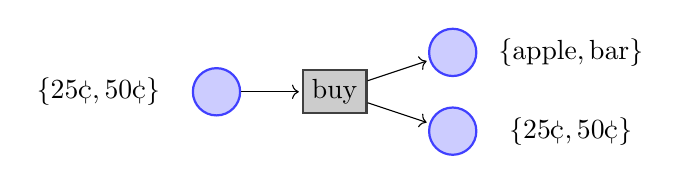
\begin{tikzpicture}
        \node (ca) at (0.5,0.5) {$\{\text{apple},\text{bar} \}$};
        \node (cb) at (0.5,-0.5) {$\{25\cent,50\cent\}$};
        \node (cc) at (-5.5,0) {$\{25 \cent,50\cent\}$};
        \node [style=place] (C) at (-1, .5) {};
        \node [style=place] (B) at (-1, -0.5) {};
        \node [style=place] (A) at (-4, 0) {};
        \node [style=transition] (tau1) at (-2.5, 0) {$\text{buy}$}
        edge [pre] (A)
        edge [post] (B)
        edge [post] (C);
\end{tikzpicture}\]
There are three species representing coins going in, food products going out, and coins going out. For each place, its set of colors is indicated next to it. The set of colors and their arc inscriptions are indicated as follows:
\begin{align*}
   25 \cent + 50 \cent & \leftmapsto  \text{a1}\mapsto (\text{apple},0)\\
  2 \cdot 50 \cent  & \leftmapsto \text{a2} \mapsto   (\text{apple},50\cent) \\
    3 \cdot 25 \cent  & \leftmapsto \text{a3} \mapsto   (\text{apple},0) \\
      25 \cent  & \leftmapsto \text{b1} \mapsto   (\text{bar},0) \\
    50 \cent  & \leftmapsto \text{b2} \mapsto   (\text{bar},25 \cent) \\
    25 \cent & \leftmapsto \text{e1} \mapsto (0,25 \cent)\\
        50 \cent & \leftmapsto \text{e2} \mapsto (0,50 \cent)
\end{align*}
The middle column gives the colors of the transition $\text{buy}$ and the columns to its left and right give the arc inscriptions for these colors on the input and output places respectively. Note that this table can be read as a span of free commutative monoids
\[\begin{tikzcd}\N[\{25 \cent, 50 \cent\} & \ar[l] \N[C
(\text{buy})] \ar[r] & \N[25 \cent, 50\cent] \oplus \N[\text{apple},\text{bar}] \end{tikzcd}\]
where $C(\text{buy})$ is the set whose elements are given by the middle column above. Let $P$ be the underlying Petri net.The above data defines a symmetric monoidal double functor $K \maps FP \to \Span(\FCMon)$. The assignment on generators of $FP$ is shown above, and this assignment is freely extended to monoidal products and composites.
\end{examples}
One advantage of phrasing colored Petri nets in categorical terms is that it gives a natural definition of morphism between colored Petri nets:

\begin{defn}\label{morphism}
    Let $K \maps FP \to \Span(\FCMon)$ and $K' \maps FP' \to \Span(\FCMon)$ be colored Petri nets. Then a \define{morphism of colored Petri nets} $(f, g, \alpha)$ is a morphism of Petri nets $(f, g) \maps P \to P'$ and a monoidal vertical transformation $\alpha$ of the following shape.
    \[
    \begin{tikzcd}
        FP 
        \ar[dd, "{F(f, g)}", swap] 
        \ar[dr, "K"{name=U}, pos=0.2]
        &\\&  
        \Span(\FCMon)
        \\
        FP'
        \ar[ur, "K'"{name=D}, swap, pos=0.15]
        & 
        \arrow[Rightarrow, from = U, to = D, shorten <=3ex, shorten >=3ex, "\alpha", swap]
    \end{tikzcd}
    \]
\end{defn}
\noindent Because this vertical transformation is monoidal, it suffices to define it on the generators of $FN$, i.e.\ the places and transitions of $N$ and not arbitrary sums of those places and transitions. Therefore, a vertical transformation as above consists of the following:
\begin{itemize}
    \item For each place $p$ a function between the color sets $\alpha_p \maps K(p) \to K'(g(p)) $. Because $FP$ is made into a double category trivially, the naturality square at this level is trivial.
    \item For each transition $\tau$, a morphism of spans i.e. a commuting diagram of the form
    \[
    \begin{tikzcd}
    K(s(\tau))\ar[d] & \ar[d]K(\tau) \ar[l] \ar[r] &\ar[d] K(t(\tau)) \\
    K'(s'(f(\tau)))) & K'(f(\tau)) \ar[l] \ar[r] & K'(t'(f(\tau)))
    \end{tikzcd}
    \]
    Because $FP$ has trivial vertical 2-cells, the naturality square at this level is also trivial.
    \item vertical transformations between double categories are required to respect composition and identities. Respecting identities is the condition that the morphism between identity spans
 \[
     \begin{tikzcd}
    K(x)\ar[d, "\alpha_x"] & \ar[d]K(x) \ar[l, equal] \ar[r, equal] &\ar[d, "\alpha_x"] K(x) \\
    K'(g(x)) & K'(g(x)) \ar[l, equal] \ar[r, equal] & K'(g(x))
    \end{tikzcd}
    \]
    has all three components given by $\alpha_x$. Respecting composition boils down to the requiring that $\alpha$ is built by extending its value on generators. For composable morphisms $\tau \maps x \to y$ and $\kappa \maps y \to z$ in $FN$, $\alpha$ gives the morphism of spans
    \[
    \begin{tikzcd}
    K(x)\ar[d, "\alpha_x"] & \ar[d, "\alpha_{K(\kappa \circ \tau)}"]K(\tau) \times_{K(y)} K(\kappa) \ar[l] \ar[r] &\ar[d, "\alpha_z"] K(z) \\
    K'(g(x)) & K'(f(\tau)) \times_{K'(g(y))} K'(f(\kappa)) \ar[l] \ar[r] & K'(g(z))
    \end{tikzcd}
    \]
    respecting composition requires that the arrow $\alpha_{K (\kappa \circ \tau))}$ is equal to the pullback of arrows $\alpha_{K(\tau)} \times_{\alpha_{K(y)}} \alpha_{K(\kappa)}$.
\end{itemize}

In \cite{lakosabstraction}, Lakos also defined morphisms of colored Petri nets. Roughly, a morphism from a colored Petri net $K=(P, T, A, C, E)$ to a colored Petri net $K'=(P', T', A', C', E')$ is a function between each set which can optionally satisfy the following properties:
\begin{itemize}
    \item {\bf Structure Respecting:} A morphism of colored Petri nets is structure respecting if it preserves arcs. This means that if an arc $a$ of $K$ connects a transition $t$ and a place $p$, then the image of this arc should connect the image of $t$ to the image of $p$. The above definition is structure respecting because it contains a morphism of the underlying Petri nets
    \item {\bf Color Respecting:} A morphism is color respecting if it sends the color on a place or a transition to a subset of the colors on the image of that place or transition. Our definition weakens this definition by requiring that there is an arbitrary monoid homomorphism between the two relevant color sets rather than an inclusion. A color respecting morphism must also preserve arc inscriptions. This is reflected in our definition by that fact that the components of $\alpha$ on the transitions are commuting diagrams of spans.
\end{itemize}
Two morphisms of colored Petri nets can be composed by composing each component separately. This forms the structure of a category.
\begin{defn}
Let \define{$\cPetri$} be the category of colored Petri nets and their morphisms.
\end{defn}
%\begin{prop}
% \label{prop:iso}
%     A morphism between Petri nets is an isomorphism if and only if both parts are isomorphisms.
% \end{prop}

% The category of colored Petri nets enjoys many nice properties
% The category of colored Petri nets can be constructed as a comma category.

% \begin{defn}
%     Let $\namedcat{cPetri}$ be the lax comma category
%     \[
%         (F \downarrow (\Set, \times) )_{\mathsf{MonLax}} 
%     \]
%     where the objects are monoidal functors $K \maps FP \to \PSet$ and the morphisms are natural transformations 
%     This is the category where objects are colored Petri nets and morphisms are the morphisms of colored Petri nets described above.
% \end{defn}

% Any uncolored Petri net can be thought of as a colored Petri net where all the color sets are singletons. Formally, any Petri net $P$ admits a constant functor $\Delta 1 \maps FP \to \PSet$. 

% This extends to a functor $T \maps \Petri \to \cPetri$ which we name the \define{trivial-coloring} functor.

% \begin{prop}
% \label{prop:embed}
%     The trivial-coloring functor gives an embedding of the category $\Petri$ of (uncolored) Petri nets into the category $\cPetri$ of colored Petri nets.
% \end{prop}

% \joe{not that this is not full because of guards\dots}

% \begin{proof}
%     Assume that there are Petri nets $P$ and $Q$ such that $TP \cong TQ$. Let \[(f, g, \alpha) \maps TP \xrightarrow{\sim} TQ\] be an isomorphism. In particular $P$ and $Q$ are isomorphic. 
    
%     Fix Petri nets $P$ and $Q$ assume $f, g \maps P \to Q$ are morphisms of Petri nets such that $Tf = Tg$. Then $Ff = Fg$, and thus $f=g$. \joe{This clearly depends on $F$ being faithful. Is this true?}
% \end{proof}

\section{Operational Semantics for Colored Petri Nets}\label{sec:unfolding}
Given a colored Petri net, there is a way to associate a category whose morphisms represent executions of your colored Petri net. To make this precise we will use the notion of step sequence. In \cite{lakosabstraction} these concepts are defined, here we adapt these definitions to our purposes:
\begin{defn}
Let $P$ be the petri net $\begin{tikzcd}T \ar[r,shift left=.5ex] \ar[r,shift right=.5ex] & \N[S] \end{tikzcd}$.
A \define{marking} of a colored Petri Net $K \maps FP \to \Span(\FCMon)$ is a pair $(m,x)$ where $m$ is a marking of the Petri $P$ and $x$ is an element of $K(m)$. A \define{step} of $K$ with \define{source} $(m,x)$ and \define{target} $(n,y)$ is a tuple $(\tau,f)$ where
\begin{itemize}
    \item $\tau$ is an element of $\N[T]$ with source given by $m$ and target given by $n$ and,
    \item $f$ is an element of the apex of $K(\tau)$ whose image under the left and right legs of $K(\tau)$ are given by $x$ and $y$ respectively.
\end{itemize}
A \define{step sequence} is a sequence of composable steps $\{(\tau_i,f_i)\}_{i=1}^{k}$. Composable means that the target of $(\tau_i,f_i)$ is equal to the source of $(\tau_{i+1},f_{i+1})$ for all $1<i<k$. In particular, setting $k=0$ gives a step sequence from every marking to itself. The source of a step sequence is defined to be the source of its first step and the target of a step sequence is the target of its last step.
\end{defn}\noindent Our categorical operational semantics will use the Grothendieck construction for displayed categories. 

\subsection{Displayed Categories}

\begin{defn}
    A \define{displayed category} over $C$ is a lax double functor 
    \[ F \maps C \to \Span(\Set)\]
\end{defn}
Displayed categories have been studied by many authors. For example, see Jean B\'enabou's lecture notes \cite{benabounotes}. The term displayed categories was first coined in  \cite{displayed}. %These are called displayed categories because they give a nice way of presenting a category $\int D$ equipped with a functor to $C$. 
The construction of $\int D$ is a generalization of the Grothendieck construction \cite{SGAI}.

\begin{defn}\label{totalcat}
For a displayed category $F \maps C \to \Span(\Set)$ its total category $\int F$ is a category where:
\begin{itemize}
    \item An object is a tuple $(c,x)$ where $c$ is an object of $C$ and $x \in F(c)$.
    \item Let $f \maps c \to d$ be a morphism in $C$ with image
    \[\begin{tikzcd}
     & F(f)\ar[dr,"b"] \ar[dl,"a",swap]& \\
    F(c) & & F(d) \end{tikzcd} \]
    then for every object $r \in F(f)$, there is a morphism $(f,r) \maps (c,a(r)) \to (d,b(r))$.
    \item For morphisms $(f,r) \maps (c,x) \to (d,y)$ and $(g,s) \maps (d,y) \to (e,z)$ their composite is defined to be $(g \circ f, t) \maps (c,x) \to (e,z)$ where $t$ is the image of the pair $(r,s)$ under the laxator of $F$
    \[F(f) \times_{F(d)} F(g) \to F(g \circ f). \]
    \end{itemize}
    $\int F$ is equipped with a functor 
    \[\Int F \to C \]
    which sends every object and morphism to its first component.
\end{defn}
Displayed categories form a category and the total category construction is a functor.
\begin{defn}
Let $F \maps C \to \Span(\Set)$ and $G \maps D \to \Span(\Set)$ be displayed categories. Then a \define{morphism of displayed categories} $(j,\alpha) \maps F \to G$ is a functor $j \maps C \to D$  and a vertical transformation between double functors filling the following diagram
\[
    \begin{tikzcd}
        C
        \ar[dd,"{j}",swap] 
        \ar[dr,"F"{name=U},pos=0.2]
        &\\&  
        \Span(\Set)
        \\
    D
        \ar[ur,"G"{name=D}, swap, pos=0.2]
        & 
        \arrow[Rightarrow, from = U, to = D, shorten <=3ex, shorten >=3ex, "\alpha", swap]
    \end{tikzcd}
    \]
 This defines a category $\define{\mathsf{Disp}}$ with composition defined as composition of vertical transformations. Let $\Cat^2$ be the category where objects are functors $D \to C$ and morphisms are commuting squares
\[\begin{tikzcd}
D \ar[d] \ar[r] & D' \ar[d]\\
C \ar[r] & C'
\end{tikzcd}
\]


\end{defn}
The following result, although very fundamental, has no reference as explained in \cite{Abramsky}. Therefore it is a result of folklore. In this paper, we remove the folklore status of this theorem and prove it in Section \ref{display}.
\begin{thm}
The total category construction gives an equivalence 
\[ \int \maps \mathsf{Disp} \xrightarrow{\sim} \Cat^2.\]
\end{thm}
% \begin{proof}
%     The following result, although very fundamental, has no reference as explained in \cite{Abramsky}. Therefore it is a result of folklore.
%     \begin{lem}\label{folklore}
%         Let $\mathsf{Disp}(C)$ be the category where objects are displayed categories over $C$ and morphisms are vertical transformations and let $\Cat/C$ be the category where objects are functors $D \to C$ and morphisms are commuting triangles. Then, the total category construction forms an equivalence
%         \[\mathsf{Disp}(C) \xrightarrow{\sim} \Cat/C\]
%     \end{lem}
%     This equivalence can be used to build the desired equivalence using the Grothendieck construction. Let $\CAT$ be the category of large categories for which $\Cat$ is an object. There is a contravariant functor
%     \[
%         \mathsf{Disp}(-) \maps \Cat^{op} \to \CAT 
%     \]
%     which sends a category $C$ to the category of displayed categories over $C$. For a functor $F \maps C \to C'$, there is a functor 
%     \[
%         \mathsf{Disp} (F) \maps \mathsf{Disp} (C') \to \mathsf{Disp}(C)
%     \] 
%     which sends a displayed category to its precomposition with $F$. Similarly, there is a functor 
%     \[
%         \Cat/(-) \maps \Cat^{op} \to \CAT 
%     \]
%     which send a category $C$ to the slice category $\Cat/C$ and a functor $F \maps C \to C'$ to the functor
%     \[\Cat/F \maps \Cat/C \to \Cat/C' \]
%     which sends a category over $C$ to its composition with $F$. One variant of the Grothendieck construction is a functor
%     \[
%         G \maps (-)/\CAT \to \CAT 
%     \]

% % The total category construction defined above forms a functor
% % \[\int \maps \mathsf{Disp} (C) \to \Cat/C. \]
% % For a vertical transformation $\alpha \maps (F \maps C \to \Span(\Set)) \Rightarrow (G \maps C \to \Span(\Set))$, there is a functor 
% % \[\int \alpha \maps \int F \to \int G \]
% % which sends
% % \begin{itemize}
% %     \item an object $(c,x)$
% % \end{itemize}
% \end{proof}
% The total category construction makes up the second half of the operational semantics for colored Petri nets. Before taking the total category, colored Petri nets must be converted into displayed categories. To this end, we seek an information preserving functor 
% \[A \maps \cPetri \to \Disp. \]
% This is accomplished by unfolding the colors of each transition and moving the monoidal structure in the fibers into the underlying Petri net.

% Suppose that $K \maps FP \to \Span(\FCMon)$ is a colored Petri net. Let $A(K) \maps FQ \to \Span(\Set)$ be the displayed category constructed as follows: Let 
% \[\tau \maps \sum x_i \to \sum y_j \]
% Then $K$ maps $\tau$ to the span
% \[\begin{tikzcd}& \ar[dl,"a",swap] K(\tau) \ar[dr,"b"] & \\
% K(x_1) \oplus K(x_2) \ldots  & & K(y_1) \oplus K(y_2) \ldots \end{tikzcd}. \]
% The free commutative monoids $K(x)$ are generated by color sets which we denote by $C(x)$. The free commutative monoid $K(x)$ has the formula
% \[ K(x) = \sum_{n \geq 0} \tilde{C(x)^n}\]
% where $\tilde{C(x)^n}$ indicates the quotient of the product $C(x)^n$ by the natural action of the symmetric group on $n$-elements. With this formula, the span corresponding to $K(\tau)$ looks like
% \[\begin{tikzcd}& \ar[dl,"a",swap] C(\tau) \ar[dr,"b"] & \\
% \sum_{n \geq 0} \tilde{C(x_1)}^n \times \sum_{n \geq 0} \tilde{C(x_2)}^n   \ldots  & &\sum_{n \geq 0} \tilde{C(y_1)}^n \times \sum_{n \geq 0} \tilde{C(y_2)}^n \ldots \end{tikzcd}. \]
% Now this span is regarded as living in $\Set$ and the commutative monoid homomorphisms $a$ and $b$ are equivalently written by their restriction to generators. For every finite sequence of natural numbers $m_1 ,\ldots, m^k$ and $n_1,\ldots,n_j$ define the set
% \[ \tau_{m_1m_2\ldots n_1 n_2 \ldots} =  a^{-1} (C(x_1)^{m_1}, C(x_2)^{m_2}, \ldots) \cap b^{-1} (C(y_1)^{n_1}, C(y_2)^{n_2}, \ldots)\]
% which captures all the colors of $\tau$ which have the same arity. The Petri net $Q$ will have one transition for every non-empty $\tau_{m_1m_2\ldots n_1 n_2 \ldots}$ with source and target having the appropriate arities. Indeed let $Q$ be a Petri net with transitions given by \[T = \{\text{ non-empty }\tau_{m_1m_2\ldots m_kn_1n_2\ldots n_j} \, | \, \tau \maps \sum_{i=1}^n x_i \to \sum_{i=1}^j y_i \text{ is a transition in $P$}\}  \]
% The source of $\tau_{m_1m_2\ldots n_1 n_2 \ldots}$, denoted $s(\tau_{m_1m_2\ldots n_1 n_2 \ldots})$, is given by $\sum m_i x_i$ and the target $t(\tau_{m_1m_2\ldots n_1 n_2 \ldots})$ is given by $\sum n_i y_i$. The strong double functor 
% \[A(K) \maps FQ \to \Span(\Set)\]
% on generating objects sends a place $p$ to its color set $C(p)$. A generating morphism, i.e. a transition $\tau_{m_1m_2\ldots n_1 n_2 \ldots} \in T$, is sent to the span
% \[
% \begin{tikzcd}& \ar[dl,"a",swap] \tau_{m_1m_2\ldots n_1 n_2 \ldots}  \ar[dr,"b"] & \\
% C(x_1)^{m_1} \times C(x_2)^{m_2} \ldots  & &C(y_1)^{n_1} \times C(y_2)^{n_2} \times  \ldots \end{tikzcd}.\]
% The assignment of $A(K)$ on the other objects and morphisms is uniquely determined by strong functoriality and strong monoidality of $A(K)$. This definition is functorial.
% \begin{defn}
% Let
% \[A \maps \cPetri \to \Disp\]
% be the functor which sends a colored Petri net $K \maps FP \to \Span(\FCMon)$ to the displayed category $A(K) \maps FQ \to \Span(\Set)$ defined above. For a morphism of colored Petri nets,
%  \[
%     \begin{tikzcd}
%         FP 
%         \ar[dd, "{F(f, g)}", swap] 
%         \ar[dr, "K"{name=U}, pos=0.2]
%         &\\&  
%         \Span(\FCMon)
%         \\
%         FP'
%         \ar[ur, "K'"{name=D}, swap, pos=0.15]
%         & 
%         \arrow[Rightarrow, from = U, to = D, shorten <=3ex, shorten >=3ex, "\alpha", swap]
%     \end{tikzcd}
%     \]
%     there is a morphism of displayed categories
%      \[
%     \begin{tikzcd}
%         FQ 
%         \ar[dd, "{A(f, g)}", swap] 
%         \ar[dr, "A(K)"{name=U}, pos=0.2]
%         &\\&  
%         \Span(\Set)
%         \\
%         FQ'
%         \ar[ur, "A(K')"{name=D}, swap, pos=0.15]
%         & 
%         \arrow[Rightarrow, from = U, to = D, shorten <=3ex, shorten >=3ex, "A(\alpha)", swap]
%     \end{tikzcd}
%     \]
% \end{defn}
% where
% \begin{itemize}
% \item $A(f,g)$ is given by $\N[g]$ on objects. Recall that for a morphism $\tau \maps \sum_{i=1}^n x_i \to \sum_{i=1}^j y_i$ the vertical transformation $\alpha$ gives commutative monoid homomorphisms
%  \[
%     \begin{tikzcd}
%     K(\sum_{i=1}^n x_i)\ar[d] & \ar[d,"\alpha_{\tau}"]K(\tau) \ar[l] \ar[r] &\ar[d] K(\sum_{i=1}^j y_i) \\
%     K'(\sum_{i=1}^n g(x_i)) & K'(f(\tau)) \ar[l] \ar[r] & K'(\sum_{i=1}^j g(y_i))
%     \end{tikzcd}
% \]

% The set $\tau_{m_1m_2\ldots m_j n_1 n_2 \ldots n_k}$ has an image under $\alpha_\tau$
% \end{itemize}
\begin{prop}
    There is a symmetric monoidal double functor 
    \[ U : \Span(\FCMon) \to \Span\]
    given by 
    \begin{itemize}
        \item  on objects $ \lambda X \mapsto \N[X]$,
        \item leaving horizontal 1-cells unchanged,
        \item on vertical 1-cells sending a function $f: X \to Y$ to the function $\N[f] : \N[X] \to \N[Y]$,
        \item and leaving vertical 2-cells unchanged.
    \end{itemize}
\end{prop}
We may compose a colored Petri net $K : FN \to \Span(\FCMon)$ with the double functor $U$ to obtained a displayed category $U \circ K : FN \to \Span$.


% Every colored Petri net gives a displayed category in a standard way. Let
% \[U \maps \FCMon \to \Set \] 
% be the forgetful functor which sends every commutative monoid to its underlying set and every monoid homomorphism to its underlying function. Then because $U$ is a right adjoint, it preserves limits and extends to a double functor 
% \[\Span(U) \maps \Span(\FCMon) \to \Span(\Set). \]
% Every colored Petri net $K \maps FN \to \Span(\FCMon)$ can be composed with $\Span(U)$ as follows
% \[\begin{tikzcd}
% FN \ar[r,"K"] & \Span(\FCMon) \ar[r,"\Span(U)"] & \Span(\Set)
% \end{tikzcd} \]
% to get a displayed category. This defines a functor 
% \[\Span(U)_* \maps \cPetri \to \Disp \]
% which sends a colored Petri net to the composite shown above and a morphism of colored Petri nets it's whiskering with $\Span(U)$. Note that because $U$ is forgetful, the functor $\Span(U)_*$ does not alter the data of colored Petri nets and their morphisms. Thus when defining the operational semantics, we will abuse notation and refer to composite 
% $\Span(U)_* \circ \int$ with the symbol $\int$.

% On a first take, it may seem like $\int K$ gives the operational semantics of $K$. However, this category overcounts the processes of $K$.

% \subsection{Colored Petri Nets are Redundant} Within a colored Petri net, there are always many ways to represent a given process. To see this let us return to the colored Petri net $K$ in Example \ref{colornet}. Suppose we want to buy both a candy bar and an apple. Then there is step 
% \[((\text{buy}, \text{a1} + \text{b1})\maps (\text{coinin},25\cent + 25\cent + 50 \cent) \to (\text{coinout},(\text{apple} +
%  \text{bar},0))\]
%  in $K$. On the other hand, the following two steps can be performed in parallel
%  \[ (\text{buy},\text{a1}) + (\text{buy},\text{b1}) \maps (\text{coinin}, 25 \cent) + (\text{coinin}, 25 \cent + 50 \cent ) \to (\text{coinout}, (\text{apple},0) + (\text{coinout},(\text{bar},0))\]
% Both of these expressions are morphisms in the category $\int K$ but they represent 
\begin{defn}\label{semantics}
The \define{categorical operational semantics functor} for colored Petri nets 
\[\int \maps \cPetri \to \Cat \]
is the composition of $\int \maps \Disp \to \Cat$ with $\Span(U) \maps \cPetri \to \Disp$.
Explicitly, for a colored Petri net $K \maps FP \to \Span(\FCMon)$ to the category $\int K$ where:
\begin{itemize}
    \item An object is a pair $(m, x)$ where $m$ is an object of $FP$ and $x$ is an element of the free commutative monoid $K(m)$.
    \item A morphism from $(m,x)$ to $(n,y)$ is a pair $(f,g)$ where $f \maps m \to n$ is a morphism in $FP$ and $g$ is an element in the apex of $F(f)$ which is mapped to $x$ and $y$ by the left and right legs of $F(f)$ respectively.
\end{itemize}
For a morphism of colored Petri nets 
   \[
    \begin{tikzcd}
        FP 
        \ar[dd, "{F(f, g)}", swap] 
        \ar[dr, "K"{name=U}, pos=0.2]
        &\\&  
        \Span(\FCMon)
        \\
        FP'
        \ar[ur, "K'"{name=D}, swap, pos=0.15]
        & 
        \arrow[Rightarrow, from = U, to = D, shorten <=3ex, shorten >=3ex, "\alpha", swap]
    \end{tikzcd}
    \]
\end{defn}
\noindent The category $\int K$ is an operational semantics for the colored Petri net $K$ in the sense that morphisms of $\int K$ represent sequences of processes which can occur in $K$. 
\begin{prop}\label{soundness}
     There is bijection between step sequences in $K$ and morphisms in $\int K$. 
\end{prop}
\begin{proof}

Each step $(\tau ,f)$ with source $(m,x)$ and target $(n,y)$ gives a morphism 
$(\tau, f) \maps (m,x) \to (n,y)$. A step sequence $\{(\tau_i,f_i)\}_{i=1}^{k}$ gives a morphism by composing all the morphisms $(\tau_i,f_i)$ with each other in the natural way.

Conversely, let $(f,g) \maps (m,x) \to (n,y)$ be a morphism in $\int K$. $FP$ is freely generated by the transitions of $P$ under $+$ and composition. Therefore $f$ will be equal to an expression built from the basic transitions using $+$ and $\circ$.
The operation $+$ satisfies the interchange law
\[ c \circ a  + d \circ b =(c+ d) \circ (a +b) \]
whenever all composites are defined. This law can be used inductively to turn $f$ into a composite of sums
\[f_1 \circ f_2 \circ \ldots \circ f_n \]
where each $f_i \maps x_i \to x_{i+1}$ is a sum of transitions in $P$.
% In particular, this tells us that for $a \maps x \to y$ and $b \maps x' \to y'$,
% \[a + b = a \circ 1_{x}+ 1_{y'} \circ b = (a + 1_{y'}) \circ (1_x  + b) \]
% This means that whenever two processes are performed in parallel an arbitrary ordering can be imposed on them. This fact can be used to inductively simplify $f$ into a composite of the form
% \[(\tau_1 + 1_{x_1}) \circ (\tau_2 + 1_{x_2}) \circ \ldots \circ (\tau_n + 1_{x_n}) \]
Because $K$ preserves composition strongly, there is an isomorphism
\[K(f) =K (f_1 \circ f_2 \ldots \circ f_n ) \cong K (f_1) \times_{K(x_2)} K(f_2) \times_{K(x_3)} \ldots \times_{K(x_{n}) } K(f_n).  \]
This isomorphism gives a way to decompose the element $g \in K(f)$ into a tuple of composable elements $g_1,g_2,\ldots, g_n$ where each $g_i$ is an element of $K(f_i)$. The pairs $(\tau_i,g_i)$ give a step sequence of $K$ which corresponds to the morphism $(f,g)$.
\end{proof}
Note that functoriality of $\int$ justifies the definition of morphism for colored Petri nets. Definition \ref{semantics} shows how morphisms of colored Petri nets lift to functors between their categories of step sequences. For a morphism of colored Petri nets $(j,\alpha) \maps K \to K'$, functoriality of $\int (j, \alpha) \maps \int K \to \int K'$ says that the mapping between step sequences induced by $\int (j,\alpha)$ respects concatenation.

\section{The Operational Semantics is Free on the Unfolding}Unfolding is a useful technique which reduces the analysis of colored Petri nets to that of ordinary Petri nets. This correspondence was first noticed by Jensen in the first volume of his book \emph{Coloured Petri nets: basic concepts, analysis methods and practical use} \cite{jensen2013coloured}. Since then, efficient algorithms have been developed for unfolding colored Petri nets \cite{systemsbio}, \cite{liu2012efficient}, \cite{kordon2006optimized}. It turns out that the operational semantics defined in the previous section is always the $\CMC$ on a some Petri net. The well-known unfolding construction gives this Petri net which generates $
int K$.
\begin{defn}\label{unfold}
For a colored Petri net $K$ with underlying Petri net $\begin{tikzcd}T \ar[r,shift left=.5ex] \ar[r,shift right=.5ex] & \N[S] \end{tikzcd}$. For a free commutative monoid $M$, let $\#M$ denote it's generating set. The \define{unfolding} of $K$ is the Petri net
\[
\begin{tikzcd} 
\UNFOLD(K) = \hat{T} \ar[r,shift left=.5ex,"\hat{s}"] \ar[r, shift right=.5ex,"\hat{t}",swap] & \N[\hat{S}]
\end{tikzcd}\]
where 
\begin{itemize}
    \item $\hat{T} = \{ (\tau, f) \, | \, \tau \in T \text{ and }f \in \# K(\tau)\}$,
    \item $\hat{S} = \{ (p, x) \,|\, p \in S \text{ and } x \in \# K(p)  \}$,
    \item $\hat{s} \maps \hat{T} \to \N[\hat{S}]$ sends a pair $(\tau,f)$ to the pair $(s(\tau), K(\tau)_{s(\tau)} (f)$ and,
    \item $\hat{t} \maps \hat{T} \to \N[\hat{S}]$ sends a pair $(\tau, f)$ to the pair $(t(\tau),K(\tau)_{t(\tau)} (f) )$.
\end{itemize}
\end{defn}
One advantage of reframing colored Petri nets in terms of category theory is that the definition of unfolding can be justified by categorical means.
The categorical semantics for Petri nets and colored Petri nets can be drawn together to get
\[
\begin{tikzcd} 
& \Petri \ar[dr,"F"] & \\
\cPetri \ar[rr,"\int",swap]  & &\CMC.
\end{tikzcd}
\]

To unfold a colored Petri net, we wish to find a functor $\mathtt{UNFOLD} \maps \cPetri \to \Petri$ such that for a colored Petri net $K$, the semantics of it's unfolding $F ( \mathtt{UNFOLD} (K) )$ matches it's original semantics $\int K$. This property says roughly that the behavior of an unfolded colored Petri must match the behavior of colored Petri net you started with. In other words $\UNFOLD$ must make the following diagram commute:
\[
\begin{tikzcd} 
& \Petri \ar[dr,"F"] & \\
\cPetri \ar[ur,"\UNFOLD"] \ar[rr,"\int",swap]  & &\CMC
\end{tikzcd}
\]
The unfolding defined above does indeed satisfy this property.

\begin{thm}\label{unfold}
    The unfolding construction extends to a functor
    \[ \UNFOLD \maps \cPetri \to \Petri\]
    satisfying the commutative diagram
\[
\begin{tikzcd} 
& \Petri \ar[dr,"F"] & \\
\cPetri \ar[ur,"\UNFOLD"] \ar[rr,"\int",swap]  & &\CMC.
\end{tikzcd}
\]
\end{thm}
\begin{proof}
$\UNFOLD$ is extended to morphisms as follows:
For a morphism of colored Petri nets $(f,g,\alpha) \maps K \to K'$, $\UNFOLD(f,g,\alpha) \maps \UNFOLD(K) \to \UNFOLD(K')$ consists of the maps
\begin{align*}
\hat{f}   \maps  \hat{T} \to \hat{T'} &\quad \quad\quad \text{and} &\hat{g}   \maps  \hat{S} \to \hat{S'}\\
      (\tau,k) \mapsto (f(\tau), \alpha_{\tau} (k) ) &  &(p,x) \mapsto (g(p), \alpha_{p} (x) )
\end{align*}
\noindent $(\hat{f},\hat{g})$ is indeed a morphism of Petri nets. Commuting with the source and target in the first component follows from $(f,g)$ being a morphism of Petri nets. Commuting with the source and target in the second component follows from $\alpha_\tau$ taking part in the commutative diagram
\[
\begin{tikzcd}
    K(s(\tau))
    \arrow[d, "\alpha_{s(\tau)}", swap]
    &
    K(\tau)
    \arrow[d, "\alpha_{\tau}"]
    \arrow[r]
    \arrow[l]
    &
    K(t(\tau))
    \arrow[d, "\alpha_{t(\tau)}"]
    \\
    K'(s'(f(\tau))
    &
    K'(f(\tau))
    \arrow[r]
    \arrow[l]
    &
    K'(t'(f(\tau)).
\end{tikzcd}
\]
Functoriality of $\UNFOLD$ follows very quickly from the definitions.

Next we show that $\UNFOLD$ respects the categorical semantics functors for $\cPetri$ and $\Petri$. For a colored Petri net $K$, we have that an isomorphism of categories
\[F \circ \UNFOLD(K) \cong \int K\]
First note that we have a bijection
\[\hat{S} \cong \coprod_{p \in S} \# K(p) \]
between $\hat{S}$ and the disjoint union of all possible colors. Therefore, the objects of $F \circ \UNFOLD (K)$ are given by
\[\N[\hat{S}] \cong \N[\coprod_{p \in S} \# K(p)] \cong \otimes_{p \in S} \N[ \# K(p) ]  \]
where the last isomorphism follows from $\N \maps \Set \to \CMon$ preserving coproducts. On the other hand,
\[\Ob \int K = \{(m,x) \, | \, m \in \N[S] \text{ and } x \in K(m) \}. \]
Because $K$ preserves the monoidal product, $K(m)$ will be isomorphic to the direct sum of commutative monoids $K(p)$ for $p \in S$. Therefore, $m$ will be a tuple of markings $(m_1, m_2, \ldots, m_k)$ where each $m_i$ is an element of the free commutative monoid on the color set for some species. An isomorphism, \[\Ob \int K \to \N[\hat{S}]\]
of commutative monoids is constructed by sending the pair $(x,(m_1,m_2,\ldots,m_k)$ to the sum $\sum_{i} m_i$ which is evidently an element of $\N[\hat{S}]$. This map is injective because $\N[\hat{S}]$ is free
\end{proof}

\begin{examples}
We can unfold the colored Petri net in Example \ref{colornet} to get the following:
\[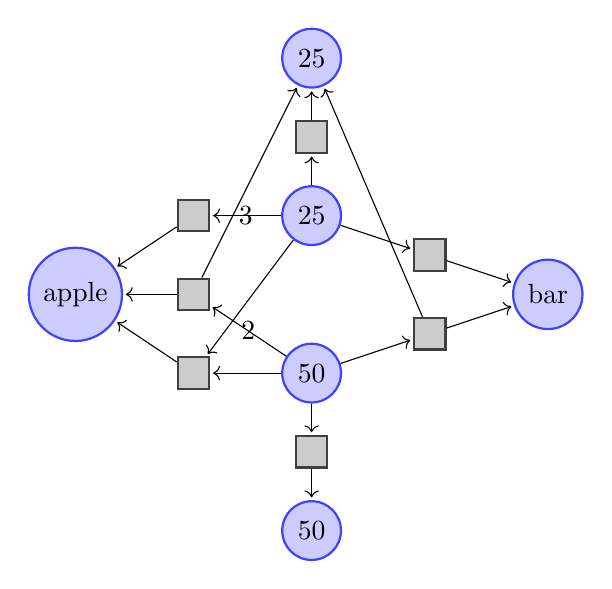
\begin{tikzpicture}
        \node [style=place] (25in) at (0,1) {25};
        \node [style=place] (50in) at (0,-1) {50};
        \node [style=place] (25out) at (0, 3) {25};
        \node [style=place] (50out) at (0,-3) {50};
        \node [style=place] (apple) at (-3,0) {apple};
        \node [style=place] (bar) at (3,0) {bar};
        \node [style=transition] (exit1) at (0, 2) {}
        edge [pre] (25in)
        edge [post] (25out);
        \node [style=transition] (exit2) at (0, -2) {}
        edge [pre] (50in)
        edge [post] (50out);
        \node [style=transition] (apple1) at (-1.5, 1) {}
        edge [pre] node {3} (25in)
        edge [post] (apple);
        \node [style=transition] (apple2) at (-1.5, -1) {}
        edge [pre]  (25in)
        edge [pre]  (50in)
        edge [post] (apple);
        \node [style=transition] (apple3) at (-1.5, 0) {}
        edge [pre] node {2} (50in)
        edge [post] (apple)
        edge [post] (25out);
        \node [style=transition] (bar1) at (1.5, .5) {}
        edge [pre] (25in)
        edge [post] (bar);
        \node [style=transition] (bar2) at (1.5, -.5) {}
        edge [pre] (50in)
        edge [post] (bar)
        edge [post] (25out);
\end{tikzpicture}\]
The categorical semantics of this Petri net...
\end{examples}


% As $F$ is fully faithful, there is an inverse
% \[F^{-1} \maps \mathrm{Im}\, F \to \Petri \]
% where $\mathrm{Im}\, F$ is the full and replete subcategory of $\CMC$ containing only the commutative monoidal categories freely generated by a Petri net. If the functor $\int$ lands in $\mathrm{Im}\,F$, then we can construct $\UNFOLD$ as the composite $F^{-1} \circ \int$. $\int$ can indeed be corestricted in this way.

% It suffices to show the following:
% \begin{itemize}
%     \item For every colored Petri net $K$ there is an ordinary Petri net $P$ such that $FP \cong \int K$.
%     \item For every morphism of colored Petri nets $((f,g) ,\alpha)) \maps K \to K'$ there is an ordinary morphism of Petri nets $(h,j) \maps P \to P'$ with $F(h,j) \maps F P \to F P'$ equal to $\int ((f,g), \alpha)) \maps \int K \to \int K'$ composed with an isomorphism on either end.
% \end{itemize}
% For the first bullet point, we will construct the Petri net \joe{ERROR}
% % $P = \hat{T} \ar[r,shift left=.5ex] \ar[r,shift right=.5ex] & \N[\hat{S}]$
%     \[
%         \hat{S} = \{ (a,x) | a \in S \text{ and } x \in K(a) \}
%     \]
%     let 
%     \[
%         \hat{T} = \{ (\tau, x, y) | \tau \in T, K(\tau)(x) = y \}
%     \]
%     and define $Q$ to be the Petri net
%     \[\begin{tikzcd}
%         \hat T 
%         \arrow[r, shift left, "\hat s"]
%         \arrow[r, shift right, "\hat t", swap]
%         & 
%         \N[\hat S].
%     \end{tikzcd}\]
%     $\hat{s}$ is the map which sends a transition $(\tau,x,y)$ to $(s(\tau),x)$ and $\hat{t}$ sends $(\tau,x,y)$ to $(t(\tau),y)$.
    
%     We construct an equivalence
%     \[
%         \alpha \maps \int K \to FQ
%     \]
%     explicitly. The objects of $FQ$ are the same; so they are sent to their counterpart in $\int K$.
% \end{proof}

% We call $Q$ the \define{unfolding} of $P$.
% \begin{examples}
% \[
% \begin{tikzpicture}
% 	\begin{pgfonlayer}{nodelayer}
%         \node [style=species] (C) at (-1, 0) {$C$};
%         \node [style=species] (B) at (-4, -0.5) {$B$};
%         \node [style=species] (A) at (-4, 0.5) {$A$};
%         \node [style=transition] (tau1) at (-2.5, 0.6) {$\;\phantom{\Big{|}}\tau_1\;$};
%         \node [style=transition] (tau2) at (-2.5, -0.7) {$\;\phantom{\Big{|}}\tau_2\;$};
% 	\end{pgfonlayer}
% 	\begin{pgfonlayer}{edgelayer}
%         \draw [style=inarrow] (A) to (tau1);
%         \draw [style=inarrow] (B) to (tau1);
%         % \draw [style=inarrow, bend right=15, looseness=1.00] (tau1) to (C);
%         \draw [style=inarrow, bend left=15, looseness=1.00] (tau1) to (C);
%         \draw [style=inarrow, bend left=15, looseness=1.00] (C) to (tau2);
%         \draw [style=inarrow, bend left=15, looseness=1.00] (tau2) to (B); 
%         \draw [style=inarrow, bend right =15, looseness=1.00] (tau2) to (B); 
% 	\end{pgfonlayer}
% \end{tikzpicture}\]

% Let $P$ denote the Petri net above. Define a coloring $K \maps FP \to \PSet$ of $P$ such that 
% \begin{align*}
%     K(A) &= \{r,g,b\}\\
%     K(B) &= \{y\}\\
%     K(C) &= \{p,d\},
% \end{align*}
% $K(\tau_1) \maps K(A) \times K(B) \to K(C)$ is given by 
% \begin{align*}
%     (r,y) &\mapsto p\\
%     (g,y) &\mapsto d\\
%     (b,y) &\mapsto \bot,
% \end{align*}
% and $K(\tau_2) \maps K(C) \to K(B) \times K(B)$ is given by 
% \begin{align*}
%     p &\mapsto (y,y)\\
%     d &\mapsto (y,y)
% \end{align*}
% \dots 
% \end{examples}
%  This construction extends to a functor.
% \begin{thm}
%     There is a functor $\mathtt{UNFOLD} \maps \cPetri \to \Petri$ which sends a colored petri net with guards $K \maps FP \to \PSet$ to to its unfolding $Q$. For a morphism of \dots
% \end{thm}

% \joe{Here we can put pseudocode for unfolding.
% for every colored place, create a place for each color, for every transition, create a copy for each tuple of input colors that doesn't get sent to the trashcan, connect them exactly as they correspond in the colored net, it will have exactly $\sum_P K_i$ places, and at worst $(\prod_P K_i) \times T$ transitions}


% \begin{algorithm}
%     unfold a colored Petri net \[K \maps FP \to \PSet \dots\] into an uncolored Petri net
% \hline
% \FOR{t \in T}
    
% \ENDFOR
% \end{algorithm}

% Categorically, colored Petri nets are the same as Petri nets. More precisely, we have the following theorem:



% \begin{thm}
% \label{thm:unfold}
%     The functor $\mathtt{UNFOLD} \maps \cPetri \to \Petri$ is left inverse to the trivial-coloring functor.
% \end{thm}

% \begin{proof}
%     \joe{what we want to show is that if we start with an uncolored Petri net $P$, then give it the trivial coloring, then unfold it, what we end up with is isomorphic to $P$.}
% \end{proof}

% \joe{one might wonder if this gives an adjunction. It doesn't because we came up with a simple counter example\dots}

% \begin{proof}[BAD PROOF]
%     It suffices to construct a functor from $\Petri$ to $\cPetri$ that is a weak right and left inverse. A weak inverse is given by the following functor
%     \begin{align*}
%         % \quad \quad 
%         U \maps \Petri &\to \cPetri
%         \\
%         P \, &\mapsto \, (\Delta 1 \maps FP \to \PSet)
%         \\
%         ((f,g) \maps P \to P') \, &\mapsto \, (f,g, \mathbf{!}) 
%     \end{align*}
%     Where $\Delta 1$ is the constant functor which sends every object to the terminal set, and every morphism $f \maps a \to b$ to the identity. The natural transformation $\mathbf{!}$ has every component given by the identity $\mathrm{id} \maps \{*\} \to \{*\}$.
    
%     Given a Petri net $P$, the unfolding of $U P$ contains no new information. Indeed, the places of $\mathtt{UNFOLD} U (P)$ are given by pairs $(a,*)$ where $a$ is a place of $P$ and $*$ is the unique element of the terminal set. The morphisms of $\mathtt{UNFOLD} \, U (P)$ are given by tuples $(\tau, *, *)$ where $\tau$ is a transition of $P$. The isomorphism
%     \[ \UNFOLD\,  U (P) \xrightarrow{\sim} P\]
%     sends $(a,*)$ to $a$ and $(\tau, * ,* )$ to $\tau$.
    
%     Given a colored Petri net 
%     \[K \maps FP \to \PSet \]
%     $U \, \UNFOLD[K] \maps F \hat{P} \to \PSet$
%     is given by functor
%     \begin{align*}
%         (a,x) \, \mapsto & \,\{*\} \\
%         (\tau,x,y) \, \mapsto & \, \mathrm{id} \maps \{*\} \to \{*\}
%     \end{align*}
%     We can define a morphism
%     \[ (f,g, \alpha) \maps U \, \UNFOLD[K] \to K\] of colored Petri nets by 
%     \begin{align*}
%         f \maps \hat{T} &\to T  \\
%         (\tau,x,y) &\mapsto \tau \\`
%         g \maps \hat{S} &\to S  \\
%         (a,x) &\mapsto  a \\
%         \alpha_a \maps \{*\} &\to K(a) \\
%         * &\mapsto  x
%     \end{align*}
%     where $\alpha_a$ is the $a$ component of the natural transformation $\alpha \maps U \, \UNFOLD[K] \Rightarrow K \circ F(f,g)$.
% \end{proof}
% Unfolding respects the semantics of a colored Petri net. This is expressed by the commutative diagram
% \jade{put this diagram in the introduction}
% \[
% \begin{tikzcd} 
% & \Petri \ar[dr,"F"] & \\
% \cPetri \ar[rr,"\int",swap] \ar[ur,"\mathtt{UNFOLD}"] & &\CMC
% \end{tikzcd}
% \]
% Roughly, this theorem says that any property of Petri nets which can suitably be expressed in categorical way is also true of colored Petri nets. In particular, this allows us to give a categorical description of the process semantics of colored Petri nets which takes advantage of the semantics for ordinary Petri nets.

% Recall that Definition \ref{unfold} defines unfolding by first taking the Grothendieck construction and then identifying a net which freely generates it. The categorical semantics of a colored Petri net should be given by the categorical semantics of it's unfolded net. However, this is the same as the free commutative monoidal category generated by the unfolded net so we can make the following definition.

% \begin{defn}
% For a colored Petri net $K \maps FP \to \PSet$, a categorical semantics functor is given by the monoidal Grothendieck construction 
% \[\int \maps \cPetri \to \CMC \]
% \end{defn}

% Functoriality of this construction is useful. It means that for a given morphism of colored Petri nets, we get a simulation of it's semantics. In practice, this means that modifications can be made to a colored Petri net in a way that is coherent with the processes it generates.

% \begin{cor}
%     The category $\cPetri$ is complete and cocomplete. \joe{we must re-examine this.}
% \end{cor}

% \begin{proof}
%     This follows from \cref{thm:equivalence} and \cref{prop:complete}.
% \end{proof}
\section{Conclusion}

Characterizing colored Petri nets categorically will allow them to be fit into the larger program of applied category theory. In particular, we conjecture that using the structured cospan construction \cite{StructuredCospans}, we can create a compositional framework for open colored Petri nets. These would be colored Petri nets which are equipped with a boundary on their inputs and outputs. One advantage of this would be a categorical description of the reachability problem for colored Petri nets as shown in \cite{OpenPetriNets}.
\appendix
% \section{Double categories}

\subsection*{Double Categories}

What follows are brief definitions of vertical transformations, monoidal double categories, and lax monoidal double functors. A more detailed exposition can be found in the work of Grandis and Par\'e \cite{GP1,GP2} \joe{missing citation}, and for monoidal double categories the work of Shulman \cite{Shulman2} \joe{missing citations}. We use `double category' to mean what earlier authors called a `pseudo double category'.

% \begin{defn}
% \label{defn:double_category}
%     A \textbf{double category} is a category weakly internal to $\Cat$. More explicitly, a double category $\mathbb{D}$ consists of:
%     \begin{itemize}
%         \item a \define{category of objects} $\mathbb{D}_0$ and a \define{category of arrows} $\mathbb{D}_1$,
%         \item  \define{source} and \define{target} functors
%         \[  
%             S,T \colon \mathbb{D}_1 \to \mathbb{D}_0 ,
%         \]
%         an \define{identity-assigning} functor
%         \[  
%             U\colon \mathbb{D}_0 \to \mathbb{D}_1 ,
%         \]
%         and a \define{composition} functor
%         \[ 
%             \odot \colon \mathbb{D}_1 \times_{\mathbb{D}_0} \mathbb{D}_1 \to \mathbb{D}_1 
%         \]
%         where the pullback is taken over $\mathbb{D}_1 \xrightarrow[]{T} \mathbb{D}_0 \xleftarrow[]{S} \mathbb{D}_1$,
%         such that
%         \[  
%             S(U_{A})=A=T(U_{A}) , \quad
%         	S(M \odot N)=SN, \quad
%             T(M \odot N)=TM, 
%         \]
%         \item natural isomorphisms called the \define{associator}
%         \[ 
%             \alpha_{N,N',N''} \maps (N \odot N') \odot N'' \xrightarrow{\sim} N \odot (N' \odot N'') , 
%         \]
%         the \define{left unitor}
%         \[		
%             \lambda_N \maps U_{T(N)} \odot N \xrightarrow{\sim} N, 
%         \]
%         and the \define{right unitor}
%         \[  
%             \rho_N \maps N \odot U_{S(N)} \xrightarrow{\sim} N 
%         \]
%         such that $S(\alpha), S(\lambda), S(\rho), T(\alpha), T(\lambda)$ and $T(\rho)$ are all identities and such that the standard coherence axioms hold: the pentagon identity for the associator and the triangle identity for the left and right unitor \cite[Sec.\ VII.1]{ML}.
%     \end{itemize}
%     If $\alpha$, $\lambda$ and $\rho$ are identities, we call $\mathbb{D}$ a \define{strict} double category.
% \end{defn}

% Objects of $\mathbb{D}_0$ are called \define{objects} and morphisms in $\mathbb{D}_0$ are called \define{vertical 1-morphisms}.  Objects of $\mathbb{D}_1$ are called \define{horizontal 1-cells} of $\mathbb{D}$ and morphisms in $\mathbb{D}_1$ are called \define{2-morphisms}.   A morphism $\alpha \maps M \to N$ in $\mathbb{D}_1$ can be drawn as a square:
% \[
% \begin{tikzpicture}[scale=1]
% \node (D) at (-4,0.5) {$A$};
% \node (E) at (-2,0.5) {$B$};
% \node (F) at (-4,-1) {$C$};
% \node (A) at (-2,-1) {$D$};
% \node (B) at (-3,-0.25) {$\Downarrow \alpha$};
% \path[->,font=\scriptsize,>=angle 90]
% (D) edge node [above]{$M$}(E)
% (E) edge node [right]{$g$}(A)
% (D) edge node [left]{$f$}(F)
% (F) edge node [above]{$N$} (A);
% \end{tikzpicture}
% \]
% where $f = S\alpha$ and $g = T\alpha$. Note that every category $C$ can be upgraded to a double category. The sets $\Ob \,C$ and $\Mor \, C$ can be regarded as categories with only identity morphisms and the structure maps (source, target, identities, and composition) extend to functors between these categories in a unique way. In this way $C$ gives a trivial double category where the only vertical morphisms and $2$-morphisms are given by identitites. 

% There are maps between double categories, and also transformations between maps:
% \begin{defn}
% \label{defn:double_functor}
% Let $\mathbb{A}$ and $\mathbb{B}$ be double categories. A \textbf{double functor} $F \maps \mathbb{A} \to \mathbb{B}$ consists of:
% \begin{itemize}
% \item functors $F_0 \maps \mathbb{A}_0 \to \mathbb{B}_0$ and $F_1 \maps \mathbb{A}_1 \to \mathbb{B}_1$ obeying the following
% equations: 
% \[S \circ F_1 = F_0 \circ S, \qquad T \circ F_1 = F_0 \circ T,\]
% \item natural isomorphisms called the \define{composition comparison}: 
% \[   \phi(N,N') \maps F_1(N) \odot F_1(N') \stackrel{\sim}{\longrightarrow} F_1(N \odot N') \]
% and the \define{identity comparison}:
% \[  \phi_{A} \maps U_{F_0 (A)} \stackrel{\sim}{\longrightarrow} F_1(U_A) \]
% whose components are globular 2-morphisms, 
% \end{itemize}
% such that the following diagram commmute:
% \begin{itemize} 
% \item a diagram expressing compatibility with the associator: 
% \[\xymatrix{ 	(F_1(N) \odot F_1(N')) \odot F_1(N'') \ar[d]_{\phi (N,N') \odot 1} \ar[r]^{\alpha} & F_1(N) \odot (F_1(N') \odot F_1(N'')) \ar[d]^{1 \odot \phi(N',N'')} \\
% 			F_1(N \odot N') \odot F_1(N'') \ar[d]_{\phi(N \odot N', N'')} & F_1(N) \odot F_1(N' \odot N'') \ar[d]^{\phi(N, N'\odot N'')}\\
% F_1((N \odot N') \odot N'') \ar[r]^{F_1(\alpha)} & F_1(N \odot (N' \odot N'')) }	\]
% \item two diagrams expressing compatibility with the left and right unitors:
% 	\[
% 	\begin{tikzpicture}[scale=1.5]
% 	\node (A) at (1,1) {$F_1(N) \odot U_{F_0(A)}$};
% 	\node (A') at (1,0) {$F_1(N) \odot F_1(U_{A})$};
% 	\node (C) at (3.5,1) {$F_1(N)$};
% 	\node (C') at (3.5,0) {$F_1(N \odot U_A)$};
% 	\path[->,font=\scriptsize,>=angle 90]
% 	(A) edge node[left]{$1 \odot \phi_{A}$} (A')
% 	(C') edge node[right]{$F_1(\rho_N)$} (C)
% 	(A) edge node[above]{$\rho_{F_1(N)}$} (C)
% 	(A') edge node[above]{$\phi(N,U_{A})$} (C');
% 	\end{tikzpicture}
% 	\]
% 	\[
% 	\begin{tikzpicture}[scale=1.5]
% 	\node (B) at (5.5,1) {$U_{F_0(B)} \odot F_1(N)$};
% 	\node (B') at (5.5,0) {$F_1(U_{B}) \odot F_1(N)$};
% 	\node (D) at (8,1) {$F_1(N)$};
% 	\node (D') at (8,0) {$F_1(U_{B} \odot N).$};
% 		\path[->,font=\scriptsize,>=angle 90]
% 		(B) edge node[left]{$\phi_{B} \odot 1$} (B')
% 	(B') edge node[above]{$\phi(U_{B},N)$} (D')
% 	(B) edge node[above]{$\lambda_{F_1(N)}$} (D)
% 	(D') edge node[right]{$F_1(\lambda_{N})$} (D);
% 	\end{tikzpicture}
% 	\]
% \end{itemize}
% If the 2-morphisms $\phi(N,N')$ and $\phi_A$ are identities for all $N,N' \in \mathbb{A}_1$ and 
% $A \in \mathbb{A}_0$, we say $F \maps \mathbb{A} \to \mathbb{B}$ is a \define{strict} double functor.  If on the other hand we drop the requirement that these 2-morphisms be invertible, we call $F$ a \define{lax} double
% functor.
% \end{defn}
	
\begin{defn}
Let $F \maps \mathbb{A} \to \mathbb{B}$ and $G \maps \mathbb{A} \to \mathbb{B}$ be lax double functors. A \define{vertical transformation} $\beta \maps F \Rightarrow G$ consists of natural transformations $\beta_0 \maps F_0 \Rightarrow G_0$ and $\beta_1 \maps F_1 \Rightarrow G_1$ (both usually written as $\beta$) such that 
		\begin{itemize}
			\item $S( \beta_M) = \beta_{SM}$ and $T(\beta_M) = \beta_{TM}$ for any object $M \in A_1$, (\joe{I don't know what kind of font you wanted but slash A isn't defined.})
			\item $\beta$ commutes with the composition comparison, and
			\item $\beta$ commutes with the identity comparison.
		\end{itemize}
\end{defn}
	
Shulman defines a 2-category $\mathbf{Dbl}$ of double categories, double functors, and vertical transformations \cite{Shulman2} \joe{Which Shulman paper?}. This has finite products.  In any 2-category with finite products we can define a pseudomonoid \cite{Monoidalbicatshopfalgebroids}, which is a categorification of the concept of monoid.  For example, a pseudomonoid in $\mathsf{Cat}$ is a monoidal category.
	
\begin{defn}
\label{defn:monoidal_double_category}
    A \textbf{monoidal double category} is a pseudomonoid in $\mathbf{Dbl}$. Explicitly, a monoidal double category is a double category equipped with double functors $\otimes \maps \mathbb{D} \times \mathbb{D} \to \mathbb{D}$ and $I \maps * \to \mathbb{D}$ where $*$ is the terminal double category, along with invertible vertical transformations called the \define{associator}:
    \[  
        A \maps \otimes \, \circ \; (1_{\mathbb{D}} \times \otimes ) \Rightarrow \otimes \; \circ \; (\otimes \times 1_{\mathbb{D}}) ,
    \]
\define{left unitor}:
\[ L\maps \otimes \, \circ \; (1_{\mathbb{D}} \times I) \Rightarrow 1_{\mathbb{D}} ,\]
and \define{right unitor}:
\[ R \maps \otimes \,\circ\; (I \times 1_{\mathbb{D}}) \Rightarrow 1_{\mathbb{D}} \]
satisfying the pentagon axiom and triangle axioms.
\end{defn}

This definition neatly packages a large quantity of information.   Namely:
\begin{itemize}
\item $\mathbb{D}_0$ and $\mathbb{D}_1$ are both monoidal categories.
\item If $I$ is the monoidal unit of $\mathbb{D}_0$, then $U_I$ is the
monoidal unit of $\mathbb{D}_1$.
\item The functors $S$ and $T$ are strict monoidal.
\item $\otimes$ is equipped with composition and identity comparisons
\[ \chi \maps (M_1\otimes N_1)\odot (M_2\otimes N_2) \stackrel{\sim}{\longrightarrow}
(M_1\odot M_2)\otimes (N_1\odot N_2)\]
\[ \mu \maps U_{A\otimes B} \stackrel{\sim}{\longrightarrow} (U_A \otimes U_B)\]
making three diagrams commute as in Def.\ \ref{defn:double_functor}.
%		\[\xymatrix{
%			((M_1\ten N_1)\odot (M_2\ten N_2)) \odot (M_3\ten N_3) \ar[r]^{\fx \odot 1} \ar[d]_{\alpha}
%			& ((M_1\odot M_2)\ten (N_1\odot N_2)) \odot (M_3\ten N_3) \ar[d]^{\fx}\\
%			(M_1\ten N_1)\odot ((M_2\ten N_2) \odot (M_3\ten N_3)) \ar[d]_{1 \odot \fx} &
%			((M_1\odot M_2)\odot M_3) \ten ((N_1\odot N_2)\odot N_3) \ar[d]^{\alpha \otimes \alpha}\\
%			(M_1\ten N_1) \odot ((M_2\odot M_3) \ten (N_2\odot N_3))\ar[r]^{\fx} &
%			(M_1\odot (M_2\odot M_3)) \ten (N_1\odot (N_2\odot N_3))}\]
%		\[\xymatrix{(M\ten N) \odot U_{C\ten D} \ar[r]^{1 \odot \fu} \ar[d]_{\rho} &
%			(M\ten N)\odot (U_C\ten U_D) \ar[d]^{\fx}\\
%			M\ten N\ar@{<-}[r]^{\rho \otimes \rho} & (M\odot U_C) \ten (N\odot U_D)}\]
%		\[\xymatrix{U_{A\ten B}\odot (M\ten N)  \ar[r]^{\fu \odot 1} \ar[d]_{\lambda} &
%			(U_A\ten U_B)\odot (M\ten N) \ar[d]^{\fx}\\
%			M\ten N\ar@{<-}[r]^{\lambda \otimes \lambda} & (U_A \odot M) \ten (U_B\odot N)}\]

\item The associativity isomorphism for $slash ten$ (\joe{slash ten is undefined}) is a vertical transformation between double functors.
%		\[\xymatrix{
%			((M_1\ten N_1)\ten P_1) \odot ((M_2\ten N_2)\ten P_2) \ar[r]^{a \odot a}\ar[d]_{\fx} &
%			(M_1\ten (N_1\ten P_1)) \odot (M_2\ten (N_2\ten P_2)) \ar[d]^{\fx}\\
%			((M_1\ten N_1) \odot (M_2\ten N_2)) \ten (P_1\odot P_2) \ar[d]_{\fx \otimes 1} &
%			(M_1\odot M_2) \ten ((N_1\ten P_1)\odot (N_2\ten P_2))\ar[d]^{1 \otimes \fx} \\
%			((M_1\odot M_2) \ten(N_1\odot N_2)) \ten (P_1\odot P_2) \ar[r]^{a} &
%			(M_1\odot M_2) \ten ((N_1\odot N_2)\ten (P_1\odot P_2))}\]
%		\[\xymatrix{
%			U_{(A\ten B)\ten C} \ar[r]^{U_{a}} \ar[d]_{\fu} & U_{A\ten (B\ten C)} \ar[d]^{\fu}\\
%			U_{A\ten B} \ten U_C \ar[d]_{\fu \otimes 1} & U_A\ten U_{B\ten C}\ar[d]^{1 \otimes \fu}\\
%			(U_A\ten U_B)\ten U_C \ar[r]^{a} & U_A\ten (U_B\ten U_C) }\]
		\item The unit isomorphisms are vertical transformations
between double functors.
%		\[\vcenter{\xymatrix{
%				(M\ten U_I)\odot (N\ten U_I)\ar[r]^{\fx}\ar[d]_{r \odot r} &
%				(M\odot N)\ten (U_I \odot U_I) \ar[d]^{1 \otimes \rho}\\
%				M\odot N \ar@{<-}[r]^{r} &
%				(M\odot N)\ten U_I }}\]
%		\[\vcenter{\xymatrix{U_{A\ten I} \ar[r]^{\fu} \ar[dr]_{U_{r}} & U_A\ten U_I \ar[d]^{r}\\
%				& U_A}}\]
%		\[\vcenter{\xymatrix{
%				(U_I\ten M)\odot (U_I\ten N)\ar[r]^{\fx} \ar[d]_{\ell \odot \ell} &
%				(U_I \odot U_I) \ten (M\odot N) \ar[d]^{\lambda \otimes 1}\\
%				M\odot N \ar@{<-}[r]^{\ell} &
%				U_I\ten (M\odot N) }}\]
%		\[\vcenter{\xymatrix{U_{I\ten A} \ar[r]^{\fu}\ar[dr]_{U_{\ell}} & U_I\ten U_A \ar[d]^{\ell}\\
%				& U_A}}\]
%		\newcounter{mondbl}
%		\setcounter{mondbl}{\value{enumi}}
	\end{itemize}


	\begin{defn}
	\label{defn:symmetric_monoidal_double_category}
A \define{braided monoidal double category} is a monoidal double
category equipped with an invertible vertical transformation
\[ \beta \maps \otimes \Rightarrow \otimes \circ \tau \]
called the \define{braiding}, where $\tau \maps \mathbb{D} \times \mathbb{D} \to \mathbb{D} \times \mathbb{D}$ is the twist double functor sending pairs in the object and arrow categories to the same pairs in the opposite order. The braiding is required to satisfy the usual two hexagon identities \cite[Sec.\ XI.1]{ML}.  If the braiding is self-inverse we say that $\mathbb{D}$ is a \define{symmetric monoidal double category}.
	\end{defn}
	
In other words:
\begin{itemize}
		\item $\mathbb{D}_0$ and $\mathbb{D}_1$ are braided (resp. symmetric) monoidal categories,
		\item the functors $S$ and $T$ are strict braided monoidal functors, and
		\item the braiding is a vertical transformation between double functors.
\end{itemize}

\begin{defn}
\label{defn:monoidal_double_functor}
    A \define{monoidal lax double functor} $F \colon \mathbb{C} \to \mathbb{D}$ between monoidal double categories $\mathbb{C}$ and $\mathbb{D}$ is a lax double functor $F \maps \mathbb{C} \to \mathbb{D}$ such that
	\begin{itemize}
		\item $F_0$ and $F_1$ are monoidal functors,
		\item $SF_1= F_0S$ and $TF_1 = F_0T$ are equations between monoidal functors, and
		\item the composition and unit comparisons $\phi(N_1,N_2) \maps F_1(N_1) \odot F_1(N_2) \to F_1(N_1\odot N_2)$ and $\phi_A \maps U_{F_0 (A)} \to F_1(U_A)$ are monoidal natural vertical transformations.
	\end{itemize}
    The monoidal lax double functor is \define{braided} if $F_0$ and $F_1$ are braided monoidal functors and \define{symmetric} if they are symmetric monoidal functors. 
    
    A fundamental example is the symmetric monoidal double category of spans.
    \begin{defn}\label{span}
    Let $\Span$ denote the double category where
\begin{itemize}
\item the category of objects is given by $\Set$: the category of sets and functions,
\item the category of morphisms $\Span_1$ has objects given by spans of functions
   \[\begin{tikzcd}A &\ar[l]X \ar[r] & B \end{tikzcd}\]
and a morphism from $\begin{tikzcd}A &\ar[l]X \ar[r] & B \end{tikzcd}$ to $\begin{tikzcd}A' &\ar[l]Y \ar[r] & B' \end{tikzcd}$ is a commuting diagram
    \[
    \begin{tikzcd}
        A\ar[d] & X \ar[r] \ar[d] \ar[l] & B \ar[d] \\
        A' & Y \ar[r] \ar[l] & B'.
    \end{tikzcd}
    \]
    \item The source and target functors $S,T \maps \Span_1 \to \Set $ send a span $\begin{tikzcd}A &\ar[l]X \ar[r] & B \end{tikzcd}$ to $A$ and $B$ respectively.
    \item The identity assigning functor $U\maps \Set \to \Span_1$ sends a set $X$ to the span $\begin{tikzcd}X &\ar[l,"1_x",swap]X \ar[r,"1_x"] & X \end{tikzcd}$.
    \item The composition functor, $\circ \maps \Span_1 \times_{\Set} \Span_1 \to \Span_1$, sends a pair of spans to their pullback and a pair of 2-morphisms to the universal map induced by the pullback.
    \item The associator, the left unitor and, the right unitor are all given by canonical isomorphisms.
\end{itemize} 
\end{defn}
\end{defn}

\section{Displayed Categories}\label{display}

% A displayed category is a way of presenting the data of a category which is in some sense torn apart. \jade{I don't know if this sentence is necessary. May I delete?} 
Technically, a displayed category is a lax functor into the category of spans. There is a procedure for constructing the category which is being displayed, called the total category. This is a generalization of the Grothendieck construction \cite{SGAI}. Like the Grothendieck construction, this gives an equivalence between the category of displayed categories and the arrow category of $\Cat$. The term ``displayed category'' was introduced in \cite{displayed}, but they have been studied before \cite{Abramsky, benabounotes}. In \cite{Abramsky}, they say that this equivalence is somewhat obvious, but a proof could not be found anywhere. 

In this appendix, we give the definition of displayed categories and the construction of the total category. In \cref{thm:intfunctor}, we prove that the construction of the total category (and its projection to the base) is functorial. In \cref{thm:Dfunctor}, we prove that there is a functorial way of constructing a displayed category from any functor. Finally, we prove the equivalence $\Disp \cong \Cat^\to$ in \cref{thm:dispequivcatarrow}. Thus, retrieving this result from the realm of folklore.

% \subsection*{Defining the categories}
% % Composition of spans given by pullback. We call a span of the form 
% % \[
% % \begin{tikzcd}
% %     &A
% %     \arrow[dl, "1_A", swap]
% %     \arrow[dr, "f"]
% %     \\
% %     A
% %     &&
% %     B
% % \end{tikzcd}\]
% % a \define{function}.

% Let $\Disp$ denote the category where
% \begin{itemize}
%     \item objects are lax double functors $F \maps X \to \Span$ where $X$ is an ordinary category upgraded to a double category with only identity tight morphisms and $2$-morphisms.
%     \item A morphism $(\phi, \alpha) \maps F \to G$ is functor $\phi \maps X \to Y$ and a double transformation $\alpha$ filling the diagram
%     \[
%     \begin{tikzcd}
%         X
%         \arrow[dr, "F"]
%         \arrow[dd, swap, "\phi"]
%         \arrow[dd, phantom, "\Downarrow \alpha", bend left = 40]
%         \\&
%         \Span
%         \\
%         Y
%         \arrow[ur, swap, "G"].
%     \end{tikzcd}\]
% \end{itemize}
% The objects of $\Disp$ are called \define{displayed categories}.

% The arrow category of $\Cat$, denoted $\Cat^\to$, where the
% \begin{itemize}
%     \item objects are functors $F \maps C \to X$
%     \item morphisms are commutative squares of functors.
%     \[\begin{tikzcd}
%         C
%         \arrow[r, "\phi_1"]
%         \arrow[d, swap, "F"]
%         &
%         D
%         \arrow[d, "G"]
%         \\
%         X
%         \arrow[r, swap, "\phi_2"]
%         &
%         Y
%     \end{tikzcd}\]
% \end{itemize}
% For convenience, we sometimes write objects in the form $[F \maps X \to Y]$, and morphisms in the form $\phi \maps [F \maps X \to Y] \to [F \maps X \to Y]$.

\subsection*{Constructing the category which is displayed}

Given a displayed category $F \maps X \to \Span$, we construct the \define{total category}, $\Int F$, where
\begin{itemize}
    \item objects are pairs $(x \in X, c \in Fx)$,
   \item morphisms are of the form $(f,g) \maps (x,c) \to (y,d)$
\end{itemize}
where $f$ is a morphism in $X$, and $g \in Ff$ such that $Ff_x(g) = c$ and $Ff_y(g) = d$. We draw such a morphism as 
\[
\begin{tikzcd}
    &
    (Ff,g)
    \arrow[dl, swap, "Ff_x"]
    \arrow[dr, "Ff_y"]
    \\
    (Fx,c)
    &&
    (Fy,d)
\end{tikzcd}\]
and we say that $g$ \define{witnesses} that $F$ relates $c$ to $d$. Composition is given by 
\[
\begin{tikzcd}
    &&
    (F(f \circ h), \psi(g,i))
    \arrow[dddll, bend right]
    \arrow[dddrr, bend left]
    \\&&
    (Ff \times_{Fy} Fh, (g,i))
    \arrow[dl]
    \arrow[dr]
    \arrow[u, "\psi"]
    \\
    &
    (Ff, g)
    \arrow[dl, "Ff_x"]
    \arrow[dr, "Ff_y", pos = 0.3]
    &&
    (Fh, i)
    \arrow[dl, swap, "Fh_y", pos = 0.3]
    \arrow[dr, swap, "Fh_z"]
    \\
    (Fx, c)
    &
    &
    (Fy, d)
    &
    &
    (Fz, e)
\end{tikzcd}\]
\joe{where we get the right commutativity of this diagram from the coherence conditions of $\psi$}.

There is a canonical projection functor $P_X \maps \Int F \to \X$ which is given by forgetting the second entry in both objects and morphisms.

\subsection*{Constructing the functor which is displayed}

Let $f \maps x \to y$ in $X$. The double transformation $\alpha$ in
\[
\begin{tikzcd}
    X
    \arrow[dr, "F"]
    \arrow[dd, swap, "\phi"]
    \arrow[dd, phantom, "\Downarrow \alpha", bend left = 40]
    \\&
    \Span
    \\
    Y
    \arrow[ur, swap, "G"]
\end{tikzcd}\]
has components which look like
\[
\begin{tikzcd}
    Fx
    \arrow[d, "\alpha_x", swap]
    &
    Ff
    \arrow[d, "\alpha_f"]
    \arrow[r, "Ff_y"]
    \arrow[l, "Ff_x", swap]
    &
    Fy
    \arrow[d, "\alpha_y"]
    \\
    G \phi x
    &
    G \phi f
    \arrow[r, "G\phi f_y", swap]
    \arrow[l, "G\phi f_x"]
    &
    G \phi y
\end{tikzcd}
\]
where $\alpha_x$ and $\alpha_y$ are the object components of $\alpha$, and $\alpha_f$ is the morphism component of $\alpha$. Commutativity of the squares gives us the following equations.
\begin{align*}
    G\phi f_y &= \alpha_y \circ Ff_y \circ \alpha_f 
    \\
    G\phi f_x &= \alpha_x \circ Ff_x \circ \alpha_f 
\end{align*}

Given a morphism $(\phi, \alpha) \maps (X, F) \to (Y, G)$ in $\Disp$, we must construct a morphism $[P_X \maps \Int F \to X] \to [P_Y \maps \Int G \to Y]$ in $\Cat^\to$. Such a morphism must be a commutative square of functors of the following form. 
\[
\begin{tikzcd}
    \Int F
    \arrow[d, "P_X", swap]
    \arrow[r, dashed]
    &
    \Int G
    \arrow[d, "P_Y"]
    \\
    X 
    \arrow[r, swap, "\phi"]
    &
    Y
\end{tikzcd}
\] 
Define the functor \[\alphahat \maps \Int F \to \Int G\] 
by 
\[
    \alphahat(x \in X, c \in F x) = (\phi x \in Y, \alpha_x c \in G \phi x)
\]
on objects, and $\alphahat(f, g) = (\phi f, \alpha_f g)$ on morphisms.
\[
\begin{tikzcd}[column sep = small]
    &
    (Ff, g)
    \arrow[dl, swap, "Ff_x"]
    \arrow[dr, "Ff_y"]
    &&&&
    (G \phi f, \alpha_f g)
    \arrow[dl, swap, "G \phi f_x"]
    \arrow[dr, "G \phi f_y"]
    \\
    (Fx, c)
    &&
    (Fy, d)
    &
    \mapsto
    &
    (G \phi x, \alpha_x c)
    &&
    (G \phi y, \alpha_y d)
\end{tikzcd}\]

\begin{lem}
    $\alphahat$ is a functor $\Int F \to \Int G$.
\end{lem}
\begin{proof}
    We check that composition is preserved.
    \begin{align*}
        \alphahat((h,i) \circ (f,g))
        &= \alphahat(h \circ f, \psi_? (g,i))
        \\&= (\phi (h \circ f), \joe{\alpha_{h \circ f} \psi_? (g,i))}
        \\&= (\phi h \circ \phi f, \joe{ \psi_?(\alpha_f g, \alpha_h i))}
        \\&= (\phi h, \alpha_h i) \circ (\phi f, \alpha_f g)
        \\&= \alphahat(h,i) \circ \alphahat(f,g) \qedhere
    \end{align*}
\end{proof}

\begin{lem}
    The following square commutes, so $(\alphahat, \phi)$ forms a morphism in $\Cat^\to$.
    \[
    \begin{tikzcd}
        \Int F
        \arrow[d, "P_X", swap]
        \arrow[r, "\alphahat"]
        &
        \Int G
        \arrow[d, "P_Y"]
        \\
        X 
        \arrow[r, swap, "\phi"]
        &
        Y
    \end{tikzcd}
    \]
\end{lem}
\begin{proof}
    Let $(x,c) \in \Int F$. Then 
    \[
        P_Y \alphahat (x,c) = P_Y(\phi x, \alpha_x(c)) = \phi x = \phi P_X(x,c).
    \]
    For $(f,g) \maps (x,c) \to (y,d)$ in $\Int F$, we get
    \[
        P_Y \alphahat (f,g) = P_Y(\phi f, \alpha_f(g)) = \phi f = \phi P_X(f,g). \qedhere
    \]
\end{proof}

\begin{prop}
\label{thm:intfunctor}
    $\Int \maps \Disp \to \Cat^\to$ is a functor
\end{prop}
\begin{proof}
    \dots
\end{proof}

\subsection*{The inverse to the total category functor}

We now define the inverse to $\Int \maps \Disp \to \Cat^\to$, which we call  $\mathscr D \maps \Cat^\to \to \Disp$. Given a functor $F \maps C \to X$, define $\mathscr DF \maps X \to \Span$ as follows. For an object $x$ of $X$, let
\[
    \mathscr DF(x) = F\inv (x) = \{c \in C |\, Fc=x\}
\]
and for a morphism $f \maps x \to y$ in $X$, let $\mathscr DF(f)$ be the span
\[
\begin{tikzcd}
    &
    F\inv f
    \arrow[dl, "s_f", swap]
    \arrow[dr, "t_f"]
    \\
    F\inv x
    &&
    F\inv y
\end{tikzcd}\]
where $F\inv f$ is the set of morphisms in $C$ that are assigned to $f$ by $F$, and $s_f$ and $t_f$ are the appropriate restrictions of the functions which assign source and target objects respectively to each morphism in $C$.

% \joe{Have to construct the laxator.}
Given a pair of composable morphisms in $C$
\[
    x \xrightarrow f y \xrightarrow g z
\]
$F$ gives us a composable pair of spans.
\[
\begin{tikzcd}
    &&
    F\inv f \times_{F\inv y} F\inv g
    \arrow[dl]
    \arrow[dr]
    \\&
    F\inv f
    \arrow[dl, "s_f", swap]
    \arrow[dr, "t_f"]
    &&
    F\inv g
    \arrow[dl, "s_g", swap]
    \arrow[dr, "t_g"]
    \\
    F\inv x
    &&
    F\inv y
    &&
    F\inv z
\end{tikzcd}\]
The apex of the composite span consists of pairs $(\phi,\psi)$ of morphisms in $C$ such that $F\phi = f$, $F\psi = g$, and $t_f(\phi) = s_g(\psi)$. So they are composable in $C$. Since $F$ is a strict functor, then $F(\psi \circ \phi) = g \circ f$, then we can choose the laxator
\[
    F_{x,y} \maps F\inv f \times_{F\inv y} F\inv g \to F(g \circ f)
\]
to be the function which gives the composite.

The unitor 
\[
\begin{tikzcd}
    &
    F\inv x
    \arrow[dl, "1", swap]
    \arrow[dd, "\mathscr DF_{1_x}"]
    \arrow[dr, "1"]
    \\
    F\inv x 
    && 
    F\inv x 
    \\&
    F\inv 1_x
    \arrow[ul, "s_{1_x}"]
    \arrow[ur, swap, "t_{1_x}"]
\end{tikzcd}
\]
is given by assigning an object $c \in F\inv x$ to its identity $1_c \in F\inv 1_x$. Since $F$ is a strict functor, then $F(1_c) = 1_x$, so this assignment makes sense.

\begin{lem}
    $\mathscr DF$ is a lax double functor $X \to \Span$.
\end{lem}
\begin{proof}
    \joe{Probably need to say a bit more about categories being monads in Span before this, or else avoid actually saying this at all.} 
    The laxator and unitor come directly from the structure which makes $C$ a monad in $\Span$. The necessary identities follow from axioms of a monad.
\end{proof}

% \joe{Given a square of functors, we define the displayed functor as follows \dots}
Given a morphism in $\Cat^\to$,
\[
\begin{tikzcd}
    C
    \arrow[d, swap, "F"]
    \arrow[r, "\phi_1"]
    &
    D
    \arrow[d, "G"]
    \\
    X
    \arrow[r, swap, "\phi_2"]
    &
    Y
\end{tikzcd}
\]
we need to construct the corresponding morphism in $\Disp$.
\[
\begin{tikzcd}
    X
    \arrow[dd, swap, "\phi_2"]
    \arrow[dd, phantom, "\Downarrow \widehat\phi", bend left = 60]
    \arrow[drr, "\mathscr DF"]
    \\&&
    \Span
    \\
    Y
    \arrow[urr, swap, "\mathscr DG"]
\end{tikzcd}
\]
The double transformation $\widehat \phi \maps \mathscr F \Rightarrow \mathscr DG \phi_2$ needs to have components of the following form.
\[
\begin{tikzcd}
    \mathscr DFx
    \arrow[d, swap, "\widehat \phi_x"]
    &
    \mathscr DFf
    \arrow[l, swap, "s_f"]
    \arrow[d, "\widehat \phi_f"]
    \arrow[r, "t_f"]
    &
    \mathscr DFy
    \arrow[d, "\widehat\phi y"]
    \\
    \mathscr DG\phi_2x
    &
    \mathscr DG\phi_2f
    \arrow[l, "s_f"]
    \arrow[r, swap, "t_f"]
    &
    \mathscr DG\phi_2y
\end{tikzcd}
\]
We abuse the labels $s_f$ and $t_f$ above. If $c$ is an object in $C$ such that $Fc = x$, then by assumption, $\phi_1c$ is an object in $D$ such that $G(\phi_1c) = \phi_2Fc = \phi_2x$. Thus we define $\widehat \phi_f (c) = \phi_1c$. If $k$ is a morphism in $C$ such that $Fk = f$, then by assumption, $\phi_1k$ is a morphism in $D$ such that $G(\phi_1k) = \phi_2Fk = \phi_2f$. Thus we define $\widehat \phi_f (k) = \phi_1k$. 

\begin{prop}
\label{thm:Dfunctor}
    $\mathscr D$ is a functor $\Cat^\to \to \Disp$.
\end{prop}
\begin{proof}
    Given composable morphisms in $\Cat^\to$
    \[
    \begin{tikzcd}
        C
        \arrow[d, swap, "F"]
        \arrow[r, "\phi_1"]
        &
        D
        \arrow[d, "G"]
        \arrow[r, "\psi_1"]
        &
        E
        \arrow[d, "H"]
        \\
        X
        \arrow[r, swap, "\phi_2"]
        &
        Y
        \arrow[r, swap, "\psi_2"]
        &
        Z
    \end{tikzcd}
    \]
    we can compose them in $\Cat^\to$ and then apply $\mathscr D$, giving
    \[
    \begin{tikzcd}
        C
        \arrow[d, swap, "F"]
        \arrow[r, "\psi_1\phi_1"]
        &
        E
        \arrow[d, "H"]
        \\
        X
        \arrow[r, swap, "\psi_2\phi_2"]
        &
        Z
    \end{tikzcd}
    \quad \mapsto \quad
    \begin{tikzcd}
        X
        \arrow[dd, swap, "\psi_2\phi_2"]
        \arrow[dd, phantom, "\Downarrow \widehat{\psi\phi}", bend left = 60]
        \arrow[drr, "\mathscr DF"]
        \\&&
        \Span
        \\
        Z
        \arrow[urr, swap, "\mathscr DH"]
    \end{tikzcd}
    \]
    % and then apply $\mathscr D$
    % \[
    % \begin{tikzcd}
    %     X
    %     \arrow[dd, swap, "\psi_2\phi_2"]
    %     \arrow[dd, phantom, "\Downarrow \widehat{\psi\phi}", bend left = 60]
    %     \arrow[drr, "\mathscr DF"]
    %     \\&&
    %     \Span
    %     \\
    %     Z
    %     \arrow[urr, swap, "\mathscr DH"]
    % \end{tikzcd}
    % \]
    or we can first apply $\mathscr D$ and then compose them in $\Disp$.
    \[
    \begin{tikzcd}
        X
        \arrow[d, swap, "\phi_2"]
        \arrow[drr, "\mathscr DF", bend left]
        \arrow[dd, phantom, "\Downarrow \widehat \phi", pos = 0.25, bend left = 70]
        \arrow[dd, phantom, "\Downarrow \widehat \psi", pos = 0.75, bend left = 70]
        \\
        Y
        \arrow[d, swap, "\psi_2"]
        \arrow[rr, "\mathscr DG"]
        &&
        \Span
        \\
        Z
        \arrow[urr, swap, "\mathscr DH", bend right]
    \end{tikzcd}
    \quad \mapsto \quad
    \begin{tikzcd}
        X
        \arrow[dd, "\psi_2 \phi_2", swap]
        \arrow[dd, phantom, "(\phi_2 \ast \widehat \psi) \widehat \phi \Downarrow", bend left = 100]
        \arrow[drrr, "\mathscr DF"]
        \\&&&
        \Span
        \\
        Z
        \arrow[urrr, swap, "\mathscr DH"]
    \end{tikzcd}
    \]
    % and then compose them in $\Disp$.
    % \[
    % \begin{tikzcd}
    %     X
    %     \arrow[dd, "\psi_2 \phi_2", swap]
    %     \arrow[dd, phantom, "(\phi_2 \ast \widehat \psi) \widehat \phi \Downarrow", bend left = 100]
    %     \arrow[drrr, "\mathscr DF"]
    %     \\&&&
    %     \Span
    %     \\
    %     Z
    %     \arrow[urrr, swap, "\mathscr DH"]
    % \end{tikzcd}
    % \]
    We must confirm that the result of these two procedures is the same. The frame is already identical as written. The morphism components of $\widehat{\psi\phi}$ are of the form
    \[\widehat{\psi\phi}_f(k) = \psi_1(\phi_1(k)).\] 
    The morphism components of $(\phi_2\ast\widehat\psi)\widehat\phi$ are of the form
    \[(\phi_2\ast\widehat\psi)\widehat\phi_f(k) = \psi_1(\phi_1(k)).\qedhere \]
\end{proof}

\subsection*{Equivalence}

Now we show that $\Int$ gives an equivalence by showing that $\mathscr D$ is a weak inverse.

\begin{thm}
\label{thm:dispequivcatarrow}
    $\mathscr D$ is a weak inverse to $\Int$. In particular, $\Disp \cong \Cat^\to$.
\end{thm}
\begin{proof}
    Let $F \maps C \to X$ be an object in $\Cat^\to$. Define $\varepsilon_F \maps \Int \mathscr DF \to C$ by 
    \begin{align*}
        \varepsilon_F(x,c) &= c\\
        \varepsilon_F(f,g) &= g.
    \end{align*}
    Composition is preserved since the decoration is given by the laxator, and the laxator for $\mathscr D$ is given by composition in $C$. Similar for identities. This is obviously surjective on objects and morphisms. If $\varepsilon_F(x,c) = \varepsilon_F(y,d)$, then $x = F(c) = F(d) = y$. Thus $\varepsilon_F$ is injective on objects. Similar for morphisms.
    
    The square
    \[
    \begin{tikzcd}
        \Int \mathscr DF
        \arrow[d, swap, "P_X"]
        \arrow[r, "\varepsilon_F"]
        &
        C
        \arrow[d, "F"]
        \\
        X
        \arrow[r, swap, "1_X"]
        &
        X
    \end{tikzcd}
    \]
    clearly commutes. We refer to the whole square as $\varepsilon_F$ as well. This is an isomorphism in $\Cat^\to$.
    
    % \joe{Have to check this is natural in $F$.}
    Given a morphism $\phi \maps F \to G$ in $\Cat^\to$, we see the square
    \[
    \begin{tikzcd}
        \Int \mathscr DF
        \arrow[r, "\varepsilon_F"]
        \arrow[d, swap, "\widehat{\widehat{\phi}}"]
        &
        C
        \arrow[d, "\phi_1"]
        \\
        \Int \mathscr DG
        \arrow[r, swap, "\varepsilon_G"]
        &
        D
    \end{tikzcd}
    \]
    commutes because 
    \begin{align*}
        \varepsilon_G \widehat{\widehat{\phi}}(x,c)
        &= \varepsilon_G (\phi_2 x, \widehat \phi (c))
        \\&= \varepsilon_G (\phi_2 x, \phi_1 (c))
        \\&= \phi_1(c)
        \\&= \phi_1 \varepsilon_F (x, c).
     \end{align*}
    Thus, the naturality square commutes.
    \[
    \begin{tikzcd}
        \Int \mathscr DF
        \arrow[r, "\varepsilon_F"]
        \arrow[d, swap, "\widehat{\widehat{\phi}}"]
        &
        F
        \arrow[d, "\phi"]
        \\
        \Int \mathscr DG
        \arrow[r, swap, "\varepsilon_G"]
        &
        G
    \end{tikzcd}
    \]
    
    Define $\eta \maps 1_\Disp \to \mathscr D\Int$ 
    \[
    \begin{tikzcd}
        X
        \arrow[rr, "F", bend left, pos = 0.55]
        \arrow[rr, phantom, "\Downarrow \eta_F"]
        \arrow[rr, swap, "\mathscr D \Int F", bend right, pos = 0.6]
        &&
        \Span
    \end{tikzcd}
    \]
    by
    \begin{align*}
        (\eta_F)_x \maps Fx & \to \mathscr D \Int F x
        \\ 
        c & \mapsto (x,c)
        \\
        (\eta_F)_x \maps Ff & \to \mathscr D \Int F f
        \\ 
        g & \mapsto (f,g).
    \end{align*}
    These are clearly isomorphisms of sets.
    
    
    \joe{Check the components are lax natural transformations.}
    
    \joe{Check it's natural.}
\end{proof}


\bibliographystyle{alpha}
\bibliography{references}

%\newpage
%\section{New Thing}

So we have a new understanding of the role that the arcs play in this story, and it informs our way of thinking about the relationship between our colored Petri nets, and those of Genovese-Spivak. 

Notice that the free commutative monoid $\N(S)$ on a set $S$ can be constructed as $\N(S) = \coprod_{n \in \N} S^n/\Sigma_n$, where $S^n$ is acted on by the symmetric group $\Sigma_n$ in the obvious way.

\begin{defn}
    A \define{single-arced net} is a Petri net of the following form.
    \[\begin{tikzcd} 
        P \maps T 
        \arrow[r, shift left, "s"] 
        \arrow[r, shift right, "t", swap] 
        &
        2^S
        \arrow[r, hookrightarrow]
        &
        \N[S]
    \end{tikzcd}\]
    A \define{condensed net} is a safe net $P$ equipped with a \joe{double??} functor of the following form.
    \[K \maps FP \to \Span(\Kl(\N))\]
\end{defn}

From a given condensed net $P$, we give a construction for a colored Petri net in the sense of Genovese-Spivak \cite{Guarded}, which will be of the following form.

\[\Khat \maps FQ \to \Span(\Set)\]

First, we must define an absolute value operation. For each $p \in S$, we define the map
\[|-| \maps \N[K(p)] \to \N\]
to return the sum of the vector's entries. For a subset $U \subseteq S$, we get
\[
    |-| \maps \N[K(U)] \cong \bigoplus_{p \in U} \left( \N[K(p)] \right) \to \bigoplus_{p \in U} \N \hookrightarrow \bigoplus_{p \in S} \N = \N[S]
\]
by taking the coproduct of the corresponding maps above and then taking the natural inclusion.

First, we give the underlying ordinary Petri net 
\begin{tikzcd} 
    Q \maps \coprod_{\tau \in T} K(\tau) 
    \arrow[r, shift left, "s'"] 
    \arrow[r, shift right, "t'", swap]
    &
    \N[S],
\end{tikzcd} 
which has
\begin{align*}
    s' &\maps \coprod_{\tau \in T} K(\tau) \to \N[S]
    \\
    t' &\maps \coprod_{\tau \in T} K(\tau) \to \N[S]
\end{align*}
defined by 
\begin{align*}
    s'(c) &= |K\tau_i(c)|
    \\
    t'(c) &= |K\tau_o(c)|
\end{align*}
where $c \in K(\tau)$.

Now we want to define the new color functor $\Khat \maps FQ \to \Span$. To each marking $\sum^n p_i$ of $Q$, we assign the set $\prod^n K(p_i)$. Recall that for a transition $\tau$ in $P$ with $s(\tau) = \sum^n p_i$ and $t(\tau) = \sum^m q_i$, $K$ gives a span in $Kl(\N)$:
\[
\begin{tikzcd}
    &
    K(\tau)
    \arrow[dl, swap, "K\tau_i"]
    \arrow[dr, "K\tau_o"]
    \\
    \N[K(s(\tau))]
    \arrow[d, swap, "\cong"]
    &&
    \N[K(t(\tau))]
    \arrow[d, "\cong"]
    \\
    \prod \N[K(p_i)]
    &&
    \prod \N[K(q_i)]
\end{tikzcd}
\]
Then for a transition $c \in K(\tau)$ of $Q$, we define $\Khat(c)$ to be the span:
\[
\begin{tikzcd}
    &
    1
    \arrow[dl, swap, "\Khat c_i"]
    \arrow[dr, "\Khat c_0"]
    \\
    \prod K(-)
    &&
    \prod K(-)
\end{tikzcd}
\]
with 
\begin{align*}
    \Khat c_i &= 
    \\
    \Khat c_o &= 
\end{align*}

\joe{I stopped here because there is a slight confusion about exactly what these values should be. The problem stems from ordered versus unordered lists of colors as the output.}

\end{document}
